\documentclass[10pt, aspectratio=169]{beamer}
\PassOptionsToPackage{table,xcdraw}{xcolor}
\usepackage{graphicx}
\usepackage{amsmath}
\usepackage{mathtools}
\usepackage{subcaption}
\usepackage{media9}
\usepackage{multicol}
\usepackage{tikz}
\usetikzlibrary{positioning, fit, arrows.meta, shapes}
\usepackage{transparent}
\usepackage{listings}
\usepackage{booktabs}
\usepackage{tabularx}
\usepackage[table,xcdraw]{xcolor}

\newcommand{\empt}[2]{$#1^{\langle #2 \rangle}$}


\usepackage{pgfplots}
\pgfplotsset{compat=1.18}

\usepackage{multirow}      % For merging rows in tables
\usepackage{colortbl}      % For coloring cells

\usepackage{fqsstyle/beamerthemefqs}
\usepackage{fqsstyle/beamercolorthemefqs}

\usepackage{comment}

\usepackage{hyperref}
\hypersetup{
    colorlinks=false,
    % linkcolor=umBlue,
    % filecolor=magenta,
    % urlcolor=cyan,
    % pdftitle={Overleaf Example},
    % pdfpagemode=FullScreen,
    }
\usepackage{xcolor}
\usepackage{amsmath}
\usepackage{wrapfig}
\usepackage{graphicx}
\usepackage{helvet}
\usepackage[T1]{fontenc}
\usepackage{tikz}
\usetikzlibrary{shapes, arrows, calc, positioning, patterns, backgrounds}
\usetikzlibrary{decorations.pathreplacing}
\usepackage{amsmath,amssymb, amsfonts}
\usepackage{lipsum}
\usepackage{datetime}
\usepackage{setspace}
\usepackage{listings}
\usepackage{fancyvrb}
%%% Local Variables:
%%% mode: latex
%%% TeX-master: "../main"
%%% End:

\renewcommand{\familydefault}{\sfdefault}
\renewcommand\mathfamilydefault{}
\newcommand{\colorbf}[1]{{\color{umGreen}\textbf{#1}}}

\newdateformat{dmydate}{%
  \twodigit{\THEDAY}~\monthname[\THEMONTH] \THEYEAR%
}

%%%%%%%%%%%%%%%%%%%%%%%%%%%%%%%%%%%%
%% eqauation
%%
\DeclareMathAlphabet{\mathbfsf}{\encodingdefault}{\sfdefault}{bx}{n}
% \renewcommand{\vec}[1]{\mathbfsf{#1}}
\newcommand{\vect}[1]{\vec{\mathbf{#1}}}
\newcommand{\brak}[1]{\langle{#1}\rangle}
\newcommand{\rbrak}[1]{\left({#1}\right)}
\newcommand{\sbrak}[1]{\left[{#1}\right]}
\newcommand{\cbrak}[1]{\left\{{#1}\right\}}
\newcommand{\abrak}[1]{\left|{#1}\right|}
\newcommand{\intInf}{\int_{-\infty}^{+\infty}}
\newcommand{\intinf}{\int_{-\infty}^{\infty}}
\newcommand{\conj}{\mathlarger{*}}%
\newcommand{\Psiconj}{\Psi^\conj}
\newcommand{\Psixt}{\Psi\rbrak{x,t}}
\newcommand{\hi}{\hat{i}}
\newcommand{\hj}{\hat{j}}
\newcommand{\hk}{\hat{k}}
\newcommand{\hx}{\hat{i}}
\newcommand{\hy}{\hat{j}}
\newcommand{\hz}{\hat{k}}
\newcommand{\vB}{\vect{B}}
\newcommand{\vE}{\vect{E}}
\newcommand{\vD}{\vect{D}}
\newcommand{\vH}{\vect{H}}
\newcommand{\curl}[1]{\vect{\nabla}\times\vect{#1}}
\newcommand{\divg}[1]{\vect{\nabla}\cdot\vect{#1}}

% quote
\newcommand{\q}[1]{``#1''}

%%% Local Variables:
%%% mode: latex
%%% TeX-master: "../main"
%%% End:


%%% Local Variables:
%%% mode: latex
%%% TeX-master: "../main"
%%% End:

\newcommand{\strong}[1]{\textcolor{umBlueLighter}{#1}}
\newcommand{\quotes}[1]{`#1'}

\mode<presentation>{%
    \usetheme{fqs}
    \usecolortheme{fqs}
}

\title[KANs]{Kolmogorov Arnold Networks}
\subtitle{Theoretical background,\\ current approaches,\\ potential next steps}

\author[T Boura \& S Konstantopoulos]{Tatiana Boura \\
  Stasinos Konstantopoulos}

\institute[]{
  
\includegraphics[height=4em]{fqsstyle/assets/ncsrd}
  
\includegraphics[height=4em]{fqsstyle/assets/deg}}

\date{28 November 2024}

\setbeamersize{text margin left=.05\pdfpagewidth,text margin right=.05\pdfpagewidth}



\begin{document}

%%%%%%%%%%%%%%%%%%%%%%%%%%%%%%%%%%%%
%%  CUSTOM TITLE PAGE: with featured image
%%
{
  \setbeamertemplate{headline}{}
  \begin{frame}
      %%%%%%%%%%%%%%%%%%%%%%
      %% Featured Image (comment or delete if not used)
      %%
      \begin{tikzpicture}[overlay, remember picture]
          \node[left=1.0cm] at (current page.1){%
              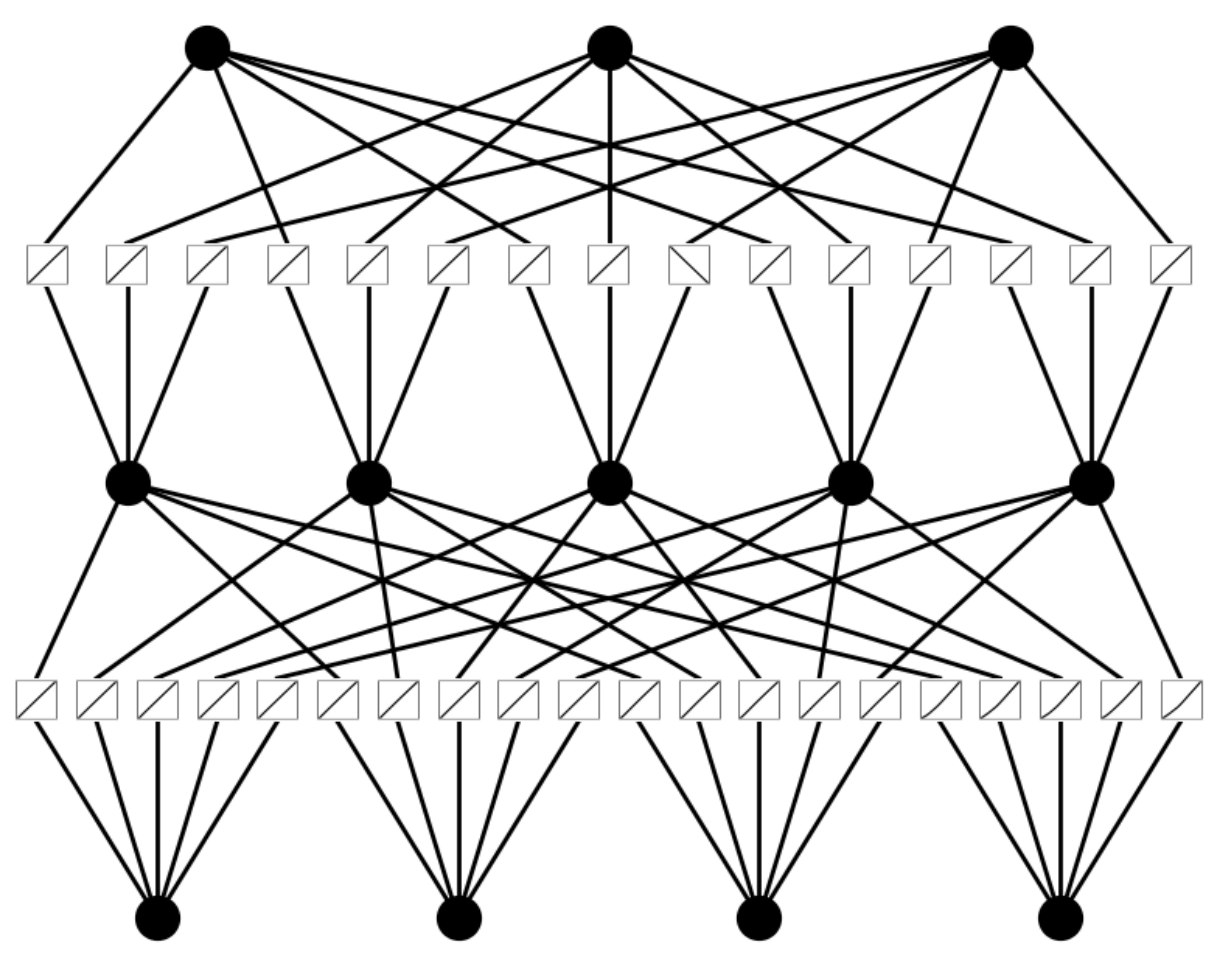
\includegraphics[width=6.5cm]{contents/images/KAN_arch_cropped}
          };
      \end{tikzpicture}
      % the title page itself
      \titlepage%
  \end{frame}
}


\section*{Introduction}
% No section page needed, I think

\begin{frame}{Outline}
  \begin{itemize}
    \setlength{\itemsep}{12pt}
  \item \strong{Part 1, Kolmogorov-Arnold Representation Theorem:}
    Historical context; proof sketch; thoughts on the theorem's impact
  \item \strong{Part 2, Kolmogorov Arnold Networks:}
    Definition; training algorithm
  \item \strong{Part 3, Why Kolmogorov Arnold Networks?}
    Motivation; expected applications
  \item \strong{Part 4, Life after KAN:}
    Extensions; DEG current work and plans
  \end{itemize}
\end{frame}

\setcounter{section}{0}

\section{Kolmogorov-Arnold Representation Theorem}
{
  \setbeamertemplate{headline}{}
  \begin{frame}
    \sectionpage%
    %\transparent{0.8} %
    %\begin{tikzpicture}[overlay,remember picture]
    %    \node[left=2cm] at (current page.2){%
    %        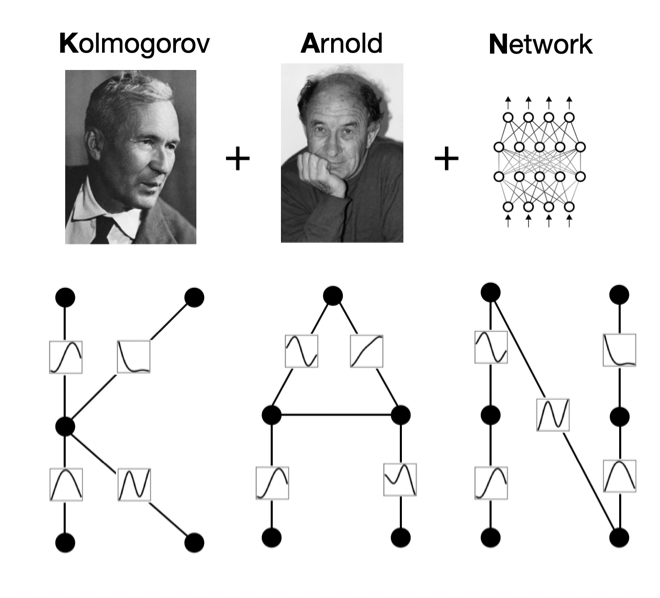
\includegraphics[width=4.5cm]{contents/images/kplusa}
    %    };
    %\end{tikzpicture}
  \end{frame}
}


%%
%% Historical context
%%

\begin{frame}[fragile]{The quadratic equation}

\begin{columns}

  \begin{column}{7.5cm}
  \begin{itemize}
  \item Methods for finding the positive roots of the
    positive-coefficients quadratic equation appear in Babylonian clay
    tablets from 21st~c. BC.
  \item In the 9th c. al-Khwarizmi proves formulas that calculate the
    positive solution(s) as functions of positive, rational coefficients
  \item In the 13th c. Yang Hui solves quadratic equations with
    negative coefficients
  \item Ren{\' e} Descartes' \emph{La G{\' e}om{\' e}trie} (1637)
    gives the quadratic formula in the form we know today
  \end{itemize}
  \end{column}

  \begin{column}{4.5cm}
  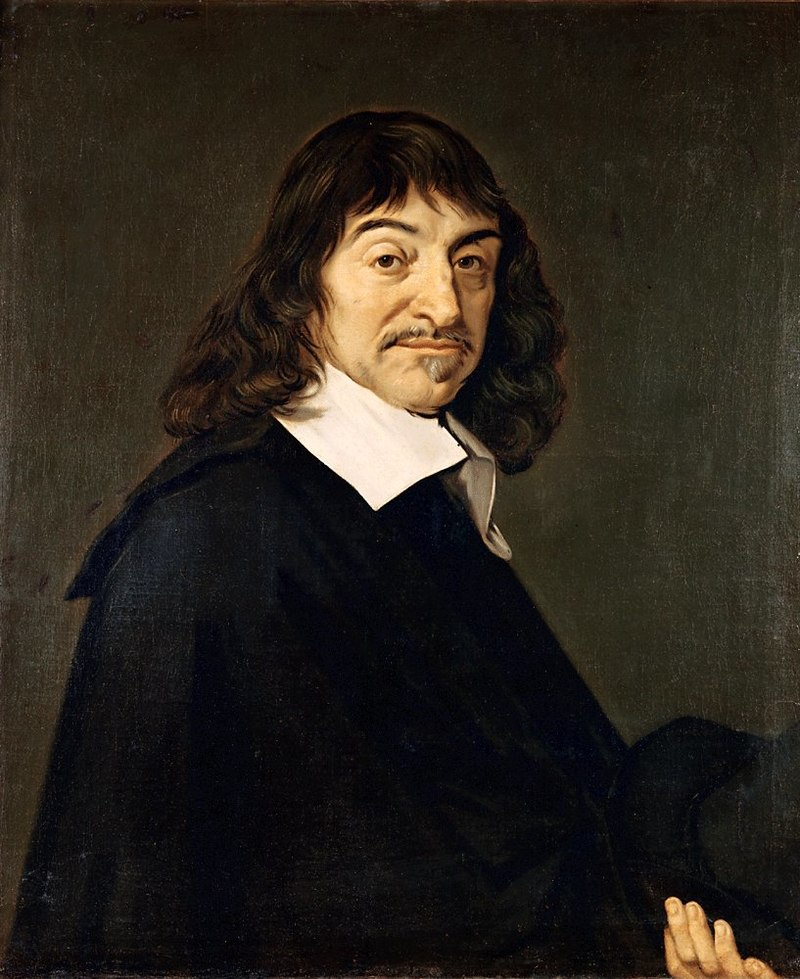
\includegraphics[width=4cm]{contents/images/descartes}
  \end{column}

\end{columns}

\end{frame}

  

\begin{frame}{The cubic and quartic equations}

\begin{columns}

  \begin{column}{7.5cm}
  \begin{itemize}
  \item Ancient solutions or almost-solutions for specific cases:
    doubling the cube, Diophantine equations, conic sections
  \item 11th c. Omar Khayyam: geometric solution, realizes multiple
    solution exist, tries and fails algebraic formulation of the
    solution
  \item Scipione del Ferro solves $x^3 + mx = n$, not
    realizing it is general
  \item Girolamo Cardano realizes (1545) del Ferro's solution and
    Lodovico Ferrari's quartic solution are general
  \item Descartes gives the modern formulas (1637)
  \end{itemize}
  \end{column}

  \begin{column}{4.5cm}
    \begin{tikzpicture}
      \node (descartes) {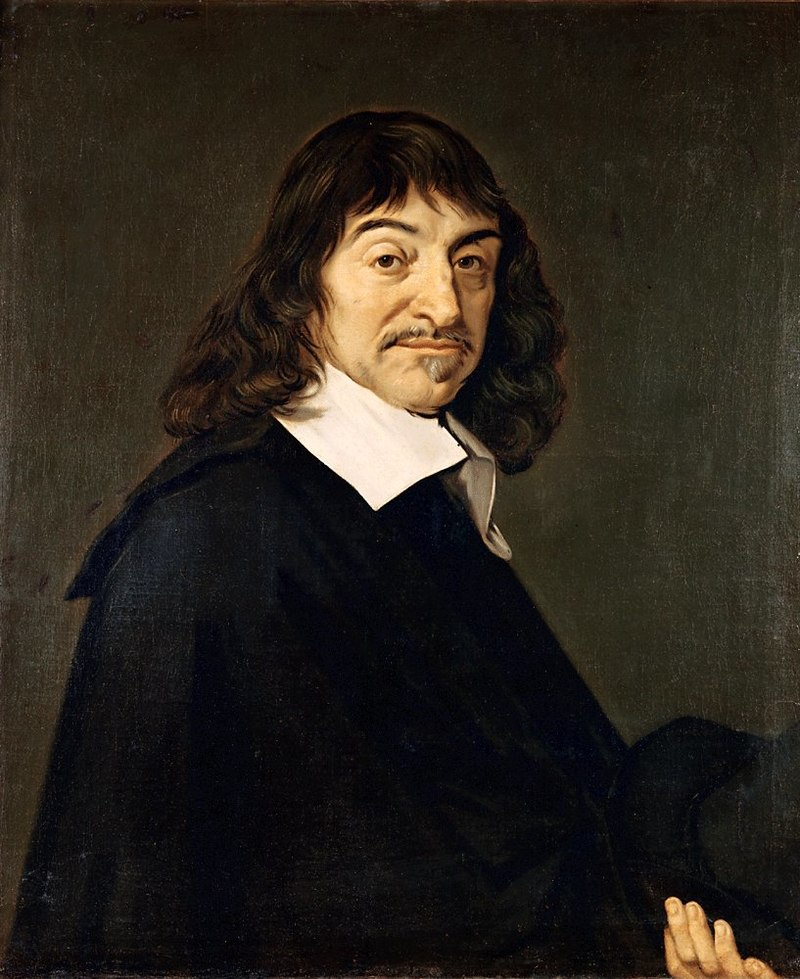
\includegraphics[width=3cm]{contents/images/descartes}};
      \node (cardano) at (descartes.south west)
            {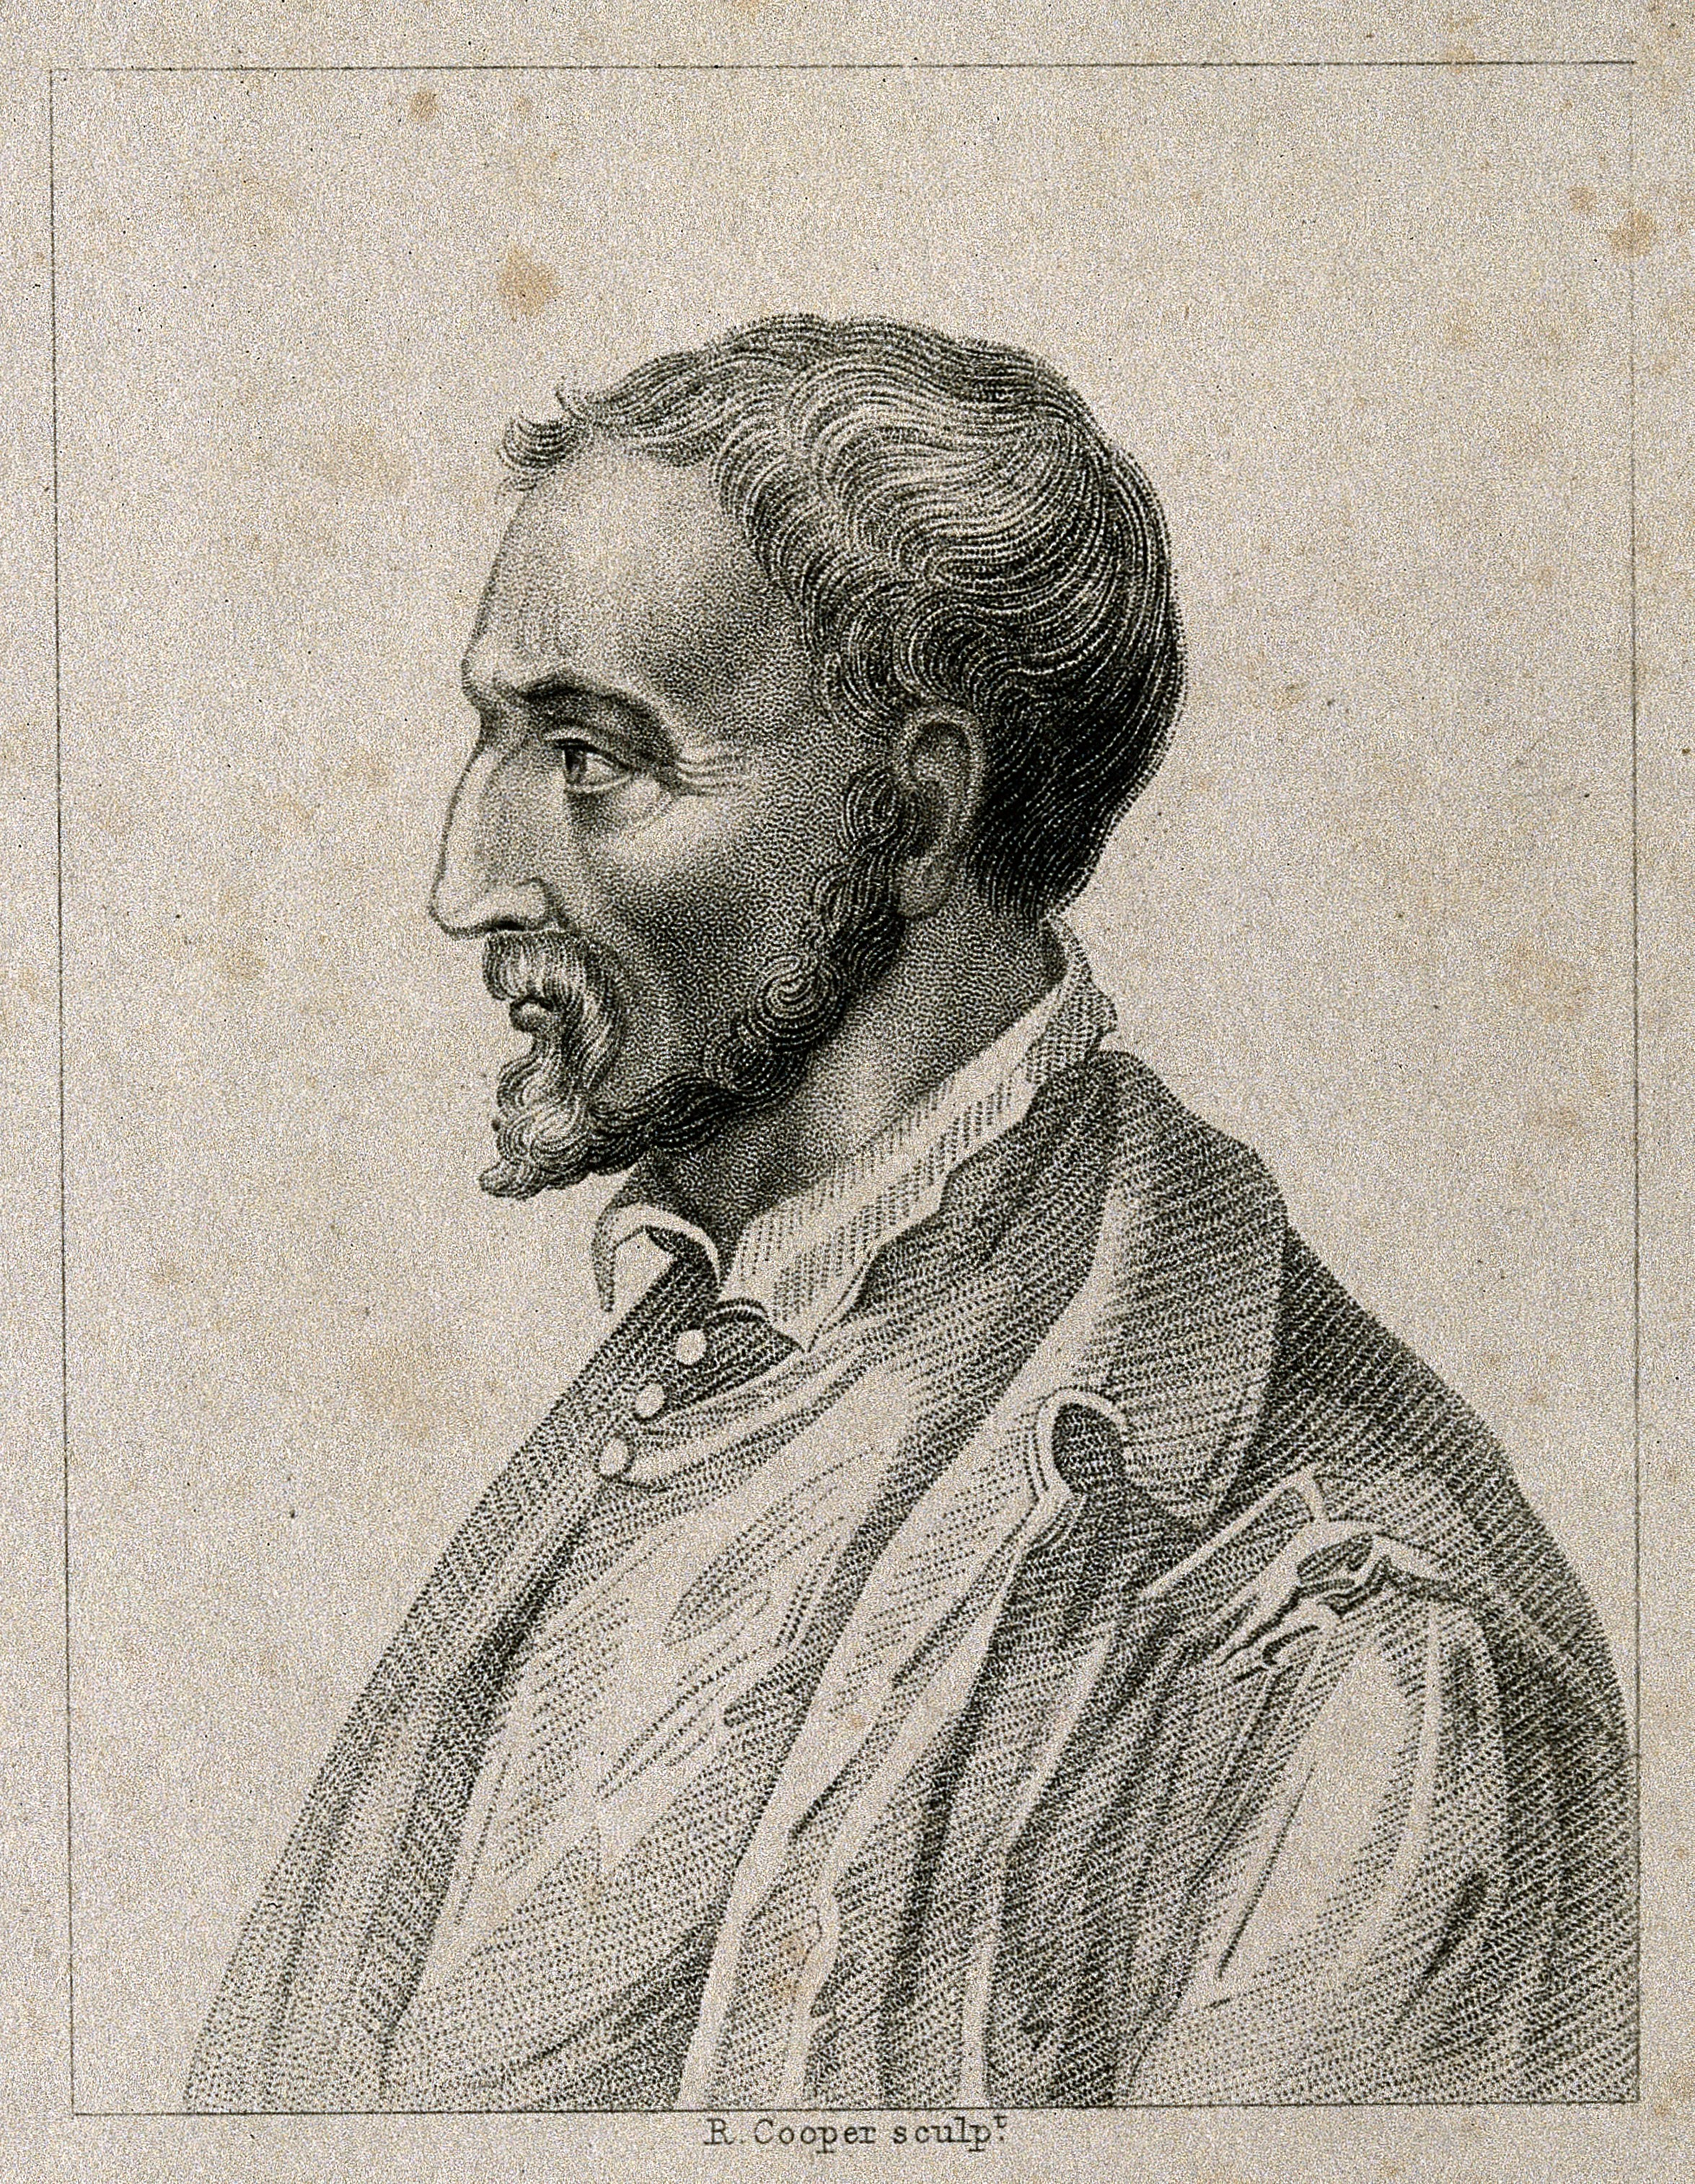
\includegraphics[width=4cm]{contents/images/cardano}};
    \end{tikzpicture}
  \end{column}

\end{columns}

\end{frame}



\begin{frame}{The end of the path}

\begin{columns}

  \begin{column}{7.5cm}
  \begin{itemize}
  \item Paolo Ruffini (1799, 1813) and Niels Henrik Abel (1824) prove
    that there is no algebraic solution to indeterminate equations of
    degree five or higher \vspace{0.5em}
  \item Galois Theory (1830, 1846) implies that there are equations of
    degree five and higher that do not have algebraic solution \vspace{0.2em}
    \begin{itemize}
    \item Almost all polynomials cannot be solved \vspace{0.1em}
    \item $x^{5}-x-1=0$ simplest unsolvable polynomial
    \end{itemize}
  \end{itemize}
  \end{column}

  \begin{column}{4.5cm}
    \begin{tikzpicture}
      \node (descartes) {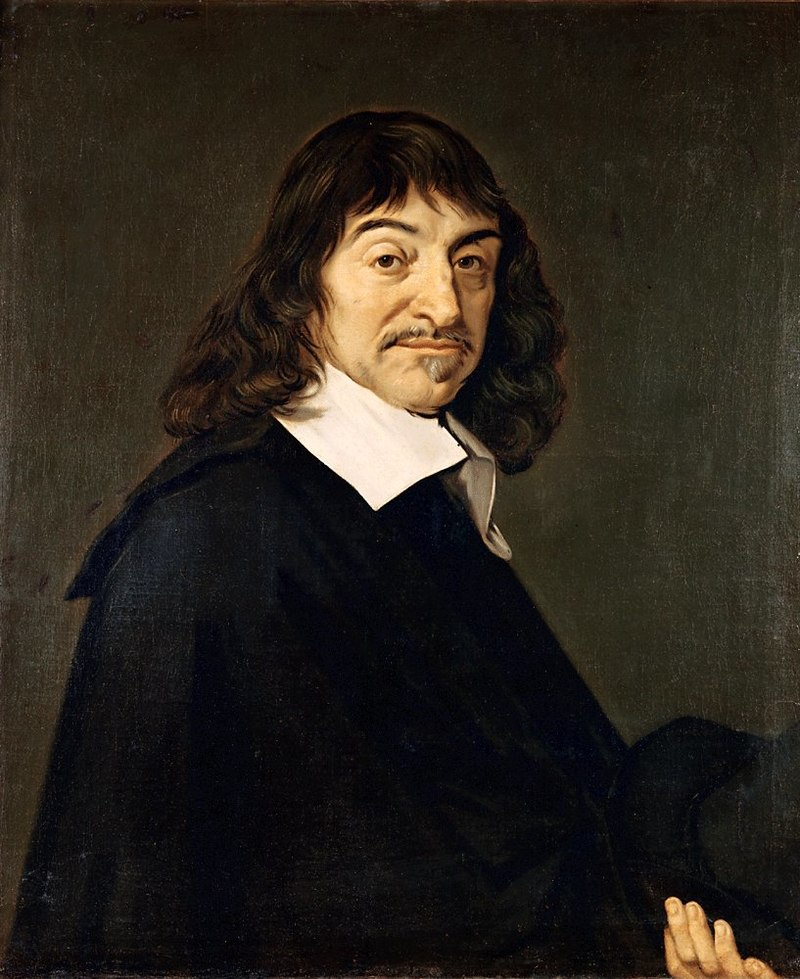
\includegraphics[width=2cm]{contents/images/descartes}};
      \node (cardano) at ([xshift=0.3cm] descartes.south west)
            {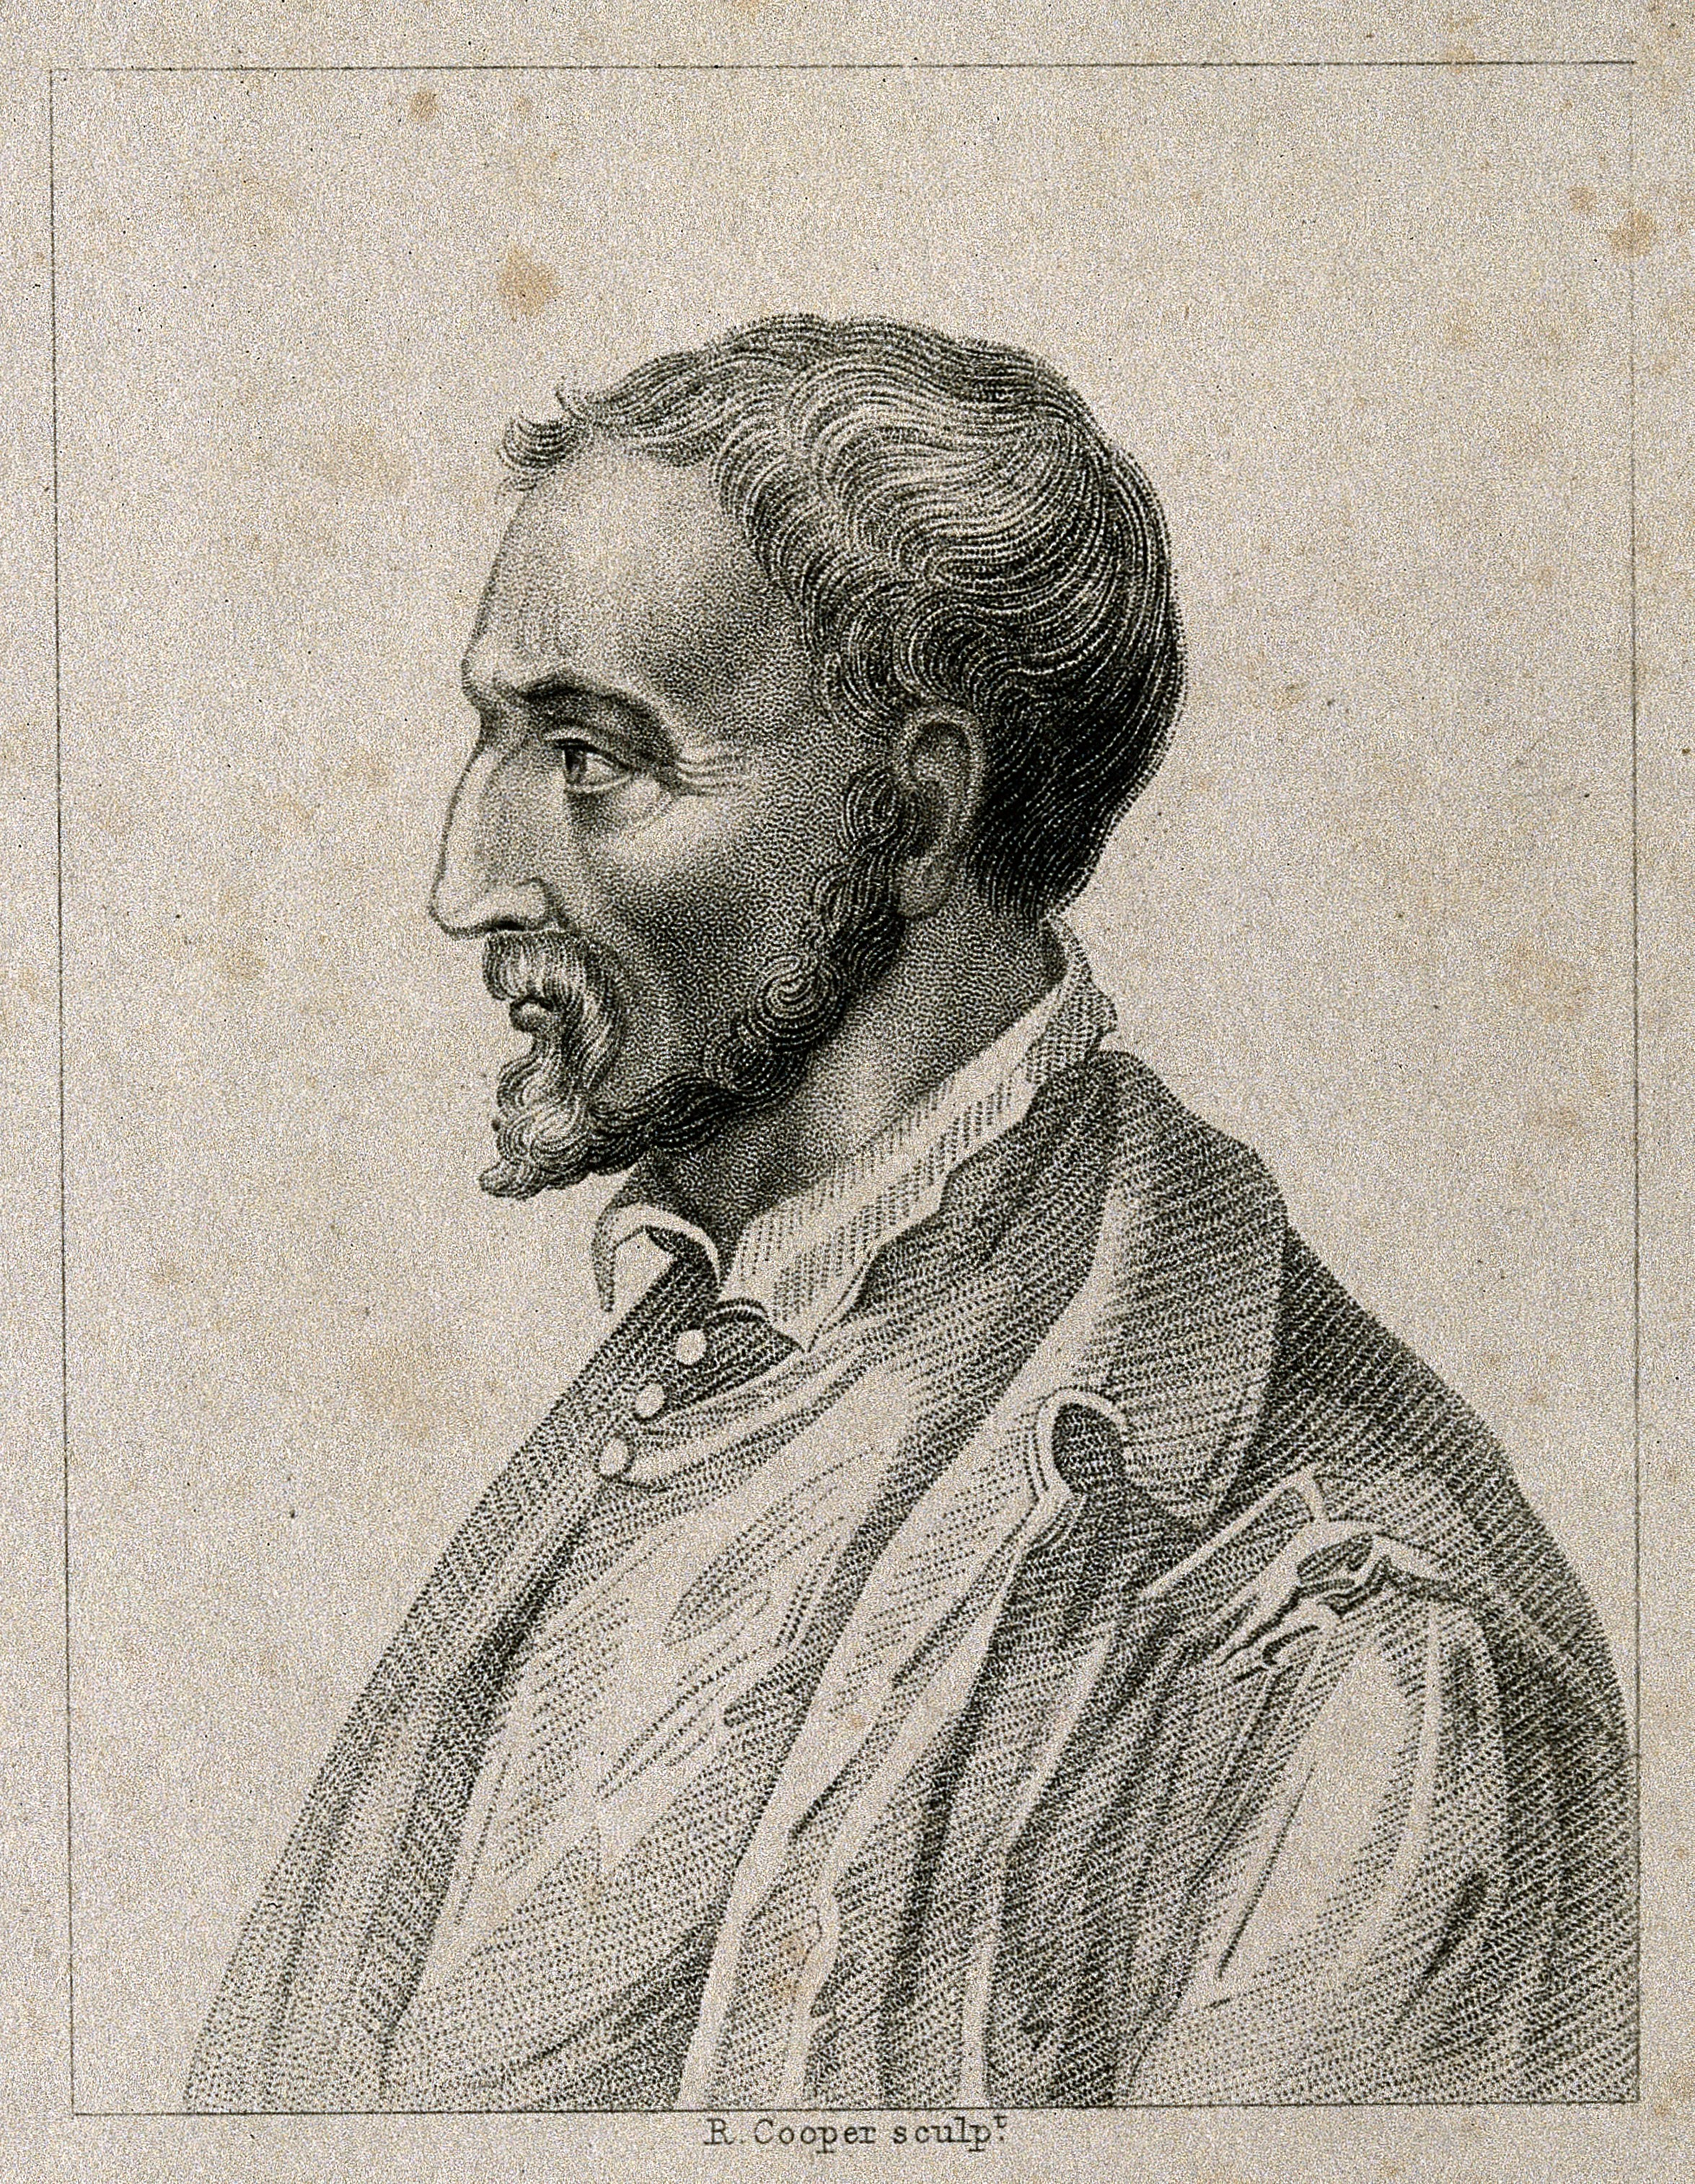
\includegraphics[width=3cm]{contents/images/cardano}};
      \node (galois) at ([xshift=0.5cm,yshift=0.5cm] cardano.south west)
            {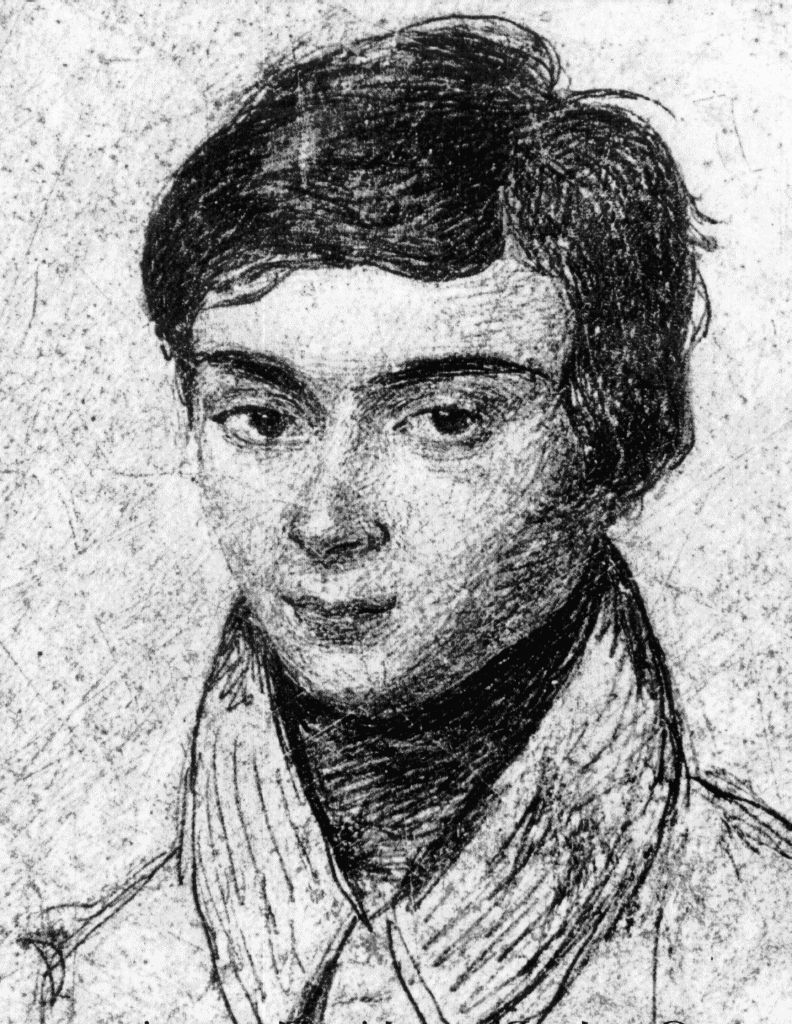
\includegraphics[width=4cm]{contents/images/galois}};
    \end{tikzpicture}
  \end{column}

\end{columns}

\end{frame}



\begin{frame}{Hilbert's 13th}

\begin{columns}

  \begin{column}{7.5cm}
  \begin{itemize}
  \item Since Tschirnhaus (1683) it is known that every 7th-degree can be
    algebraically reduced to $x^{7}+ax^{3}+bx^{2}+cx+1=0$
  \item Algebraic solutions are functions of three variables
  \item \emph{Can this be expressed as the composition of a finite number
    of two-variable functions?} (Hilbert 1900, 1902)
  \item Following up on a series of post-Galois results on trying to
    understand high-order algebraic polynomial equations
  \end{itemize}
  \end{column}

  \begin{column}{4.5cm}
    \begin{tikzpicture}
      \node (cardano) {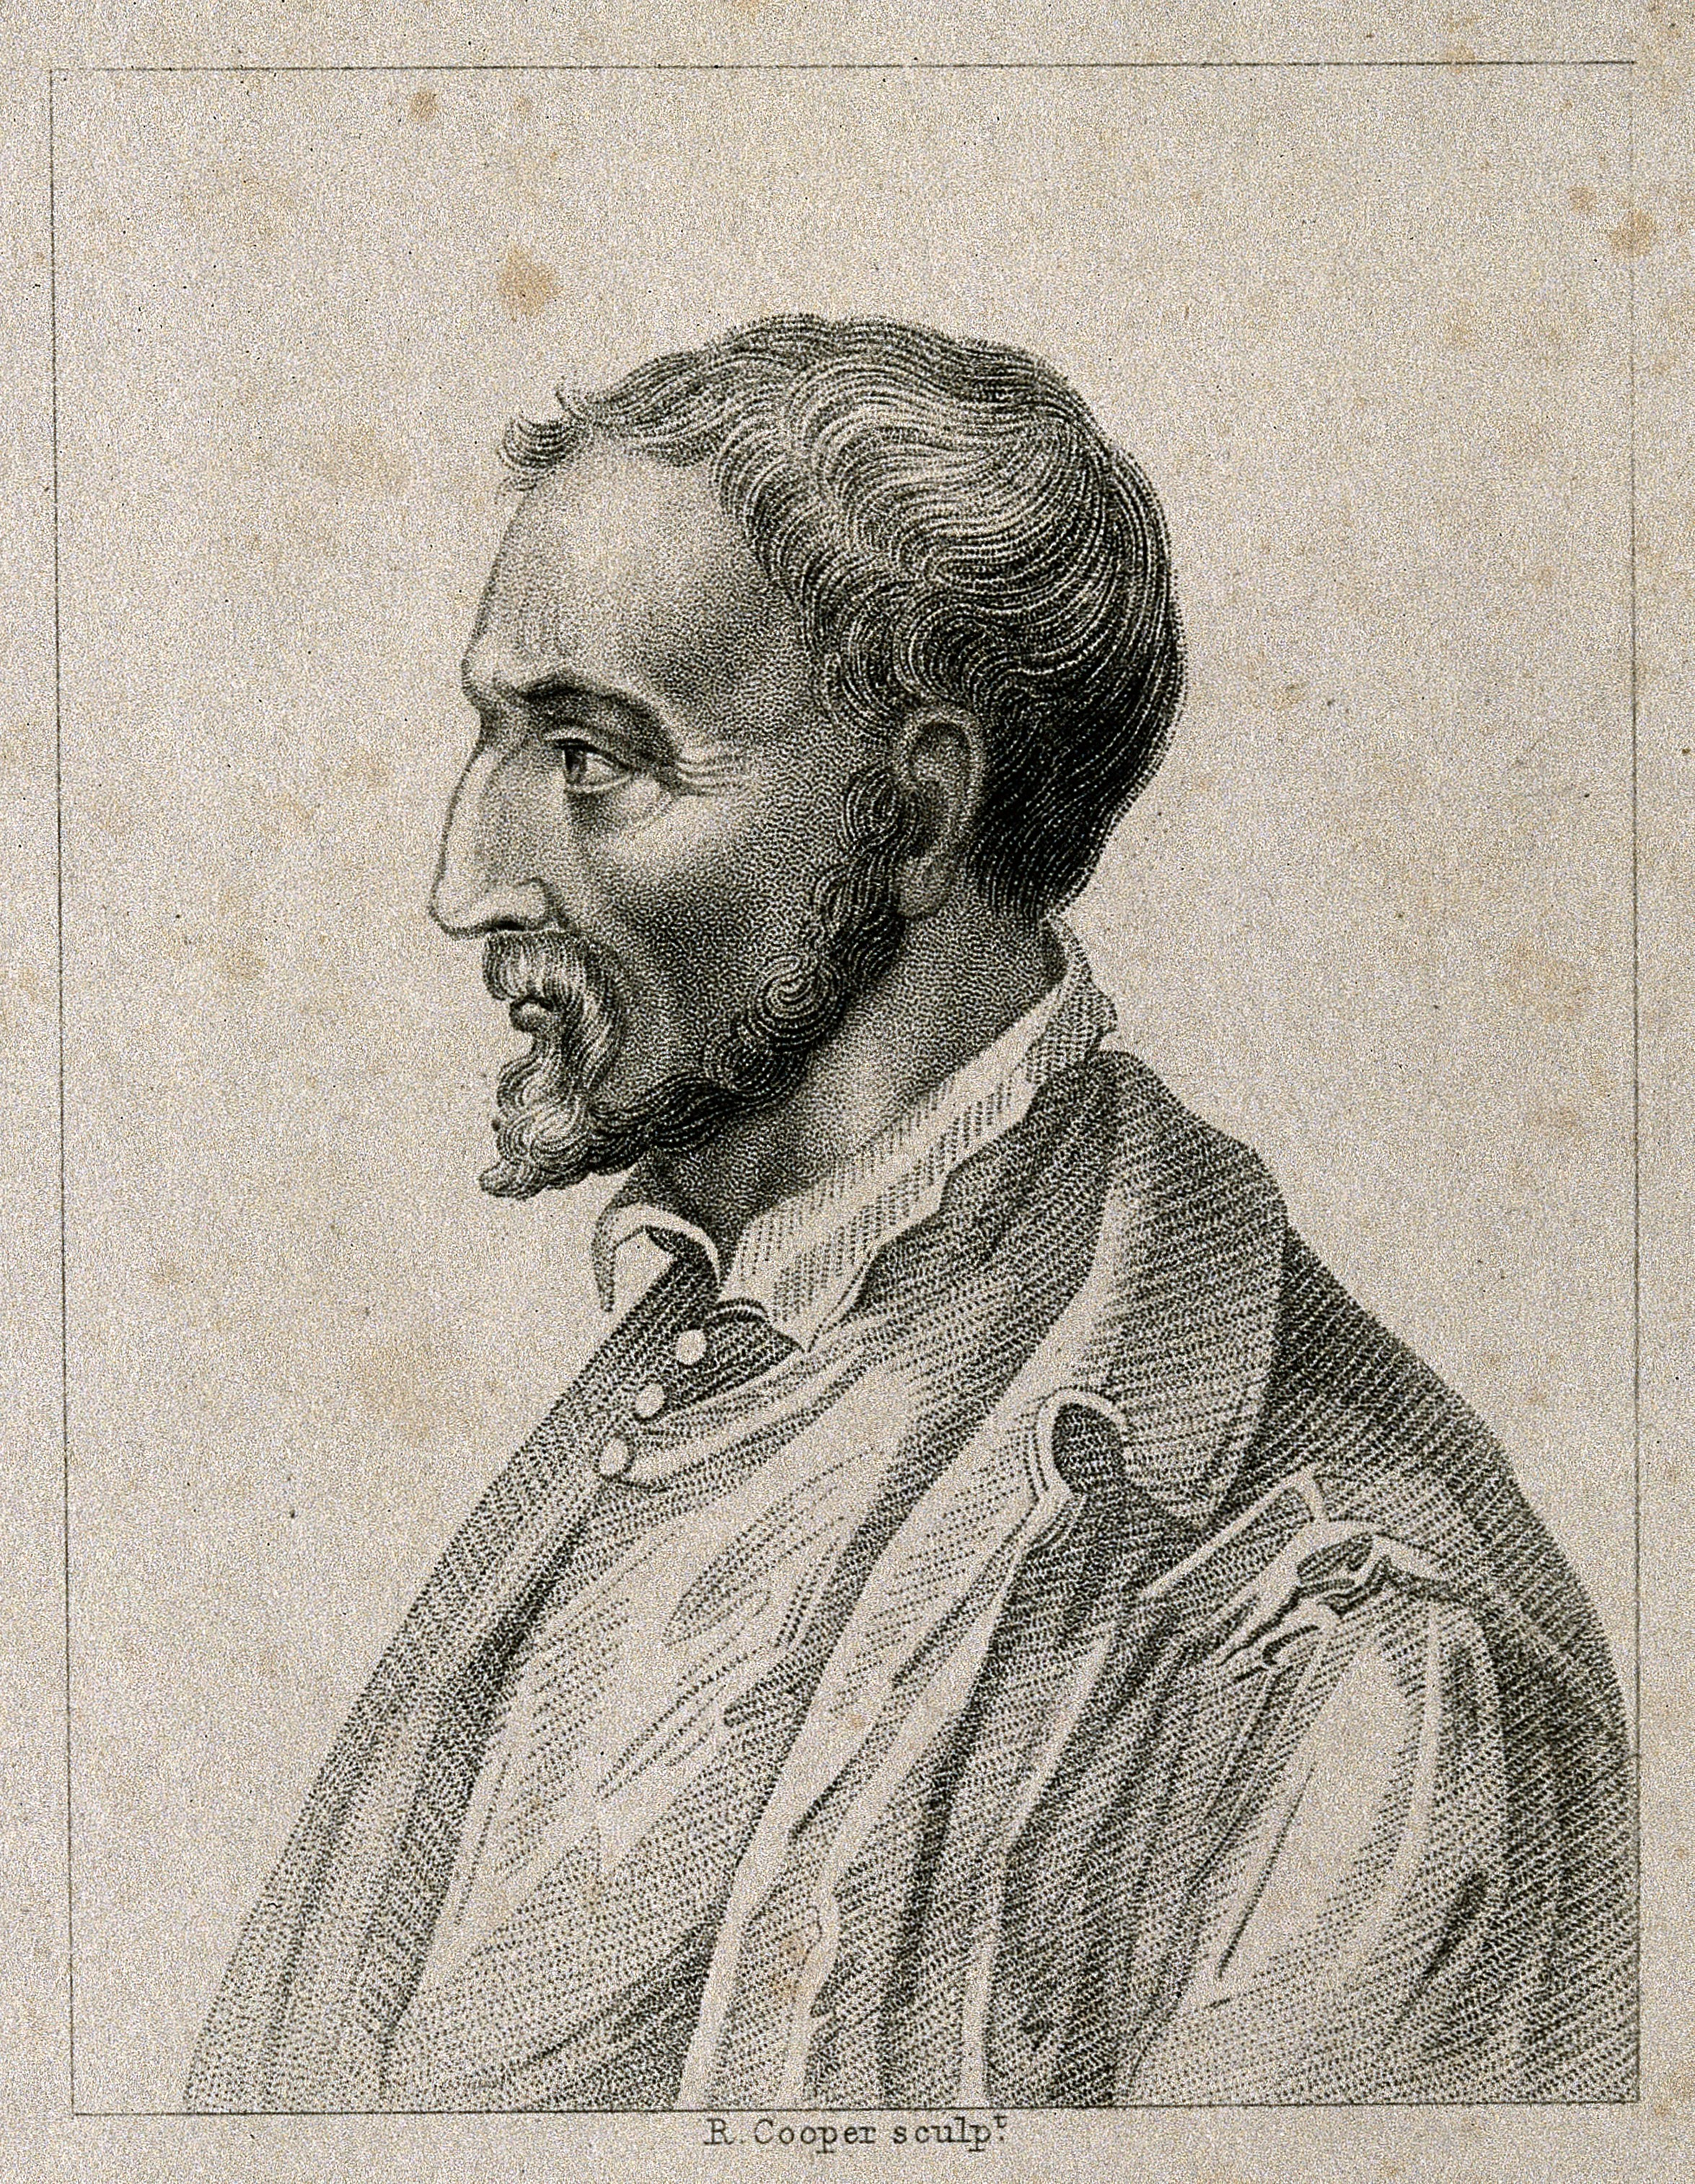
\includegraphics[width=2cm]{contents/images/cardano}};
      \node (galois) at ([xshift=0.3cm] cardano.south west)
            {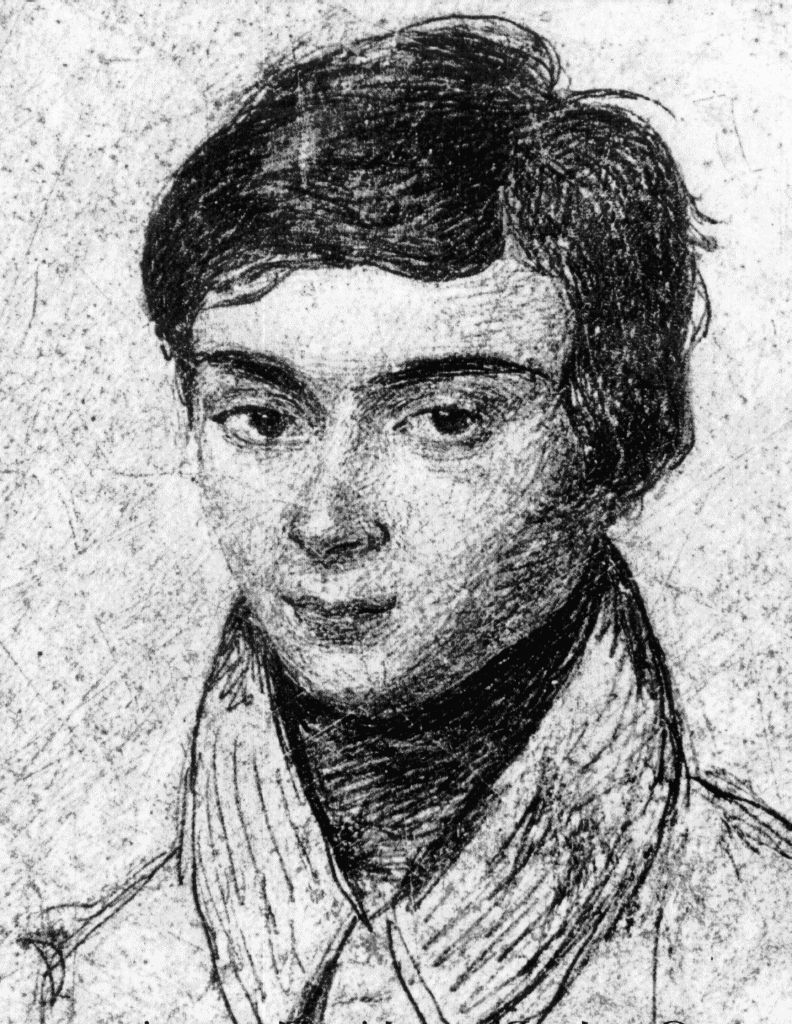
\includegraphics[width=3cm]{contents/images/galois}};
      \node (hilbert) at ([xshift=0.5cm,yshift=0.5cm] galois.south west)
            {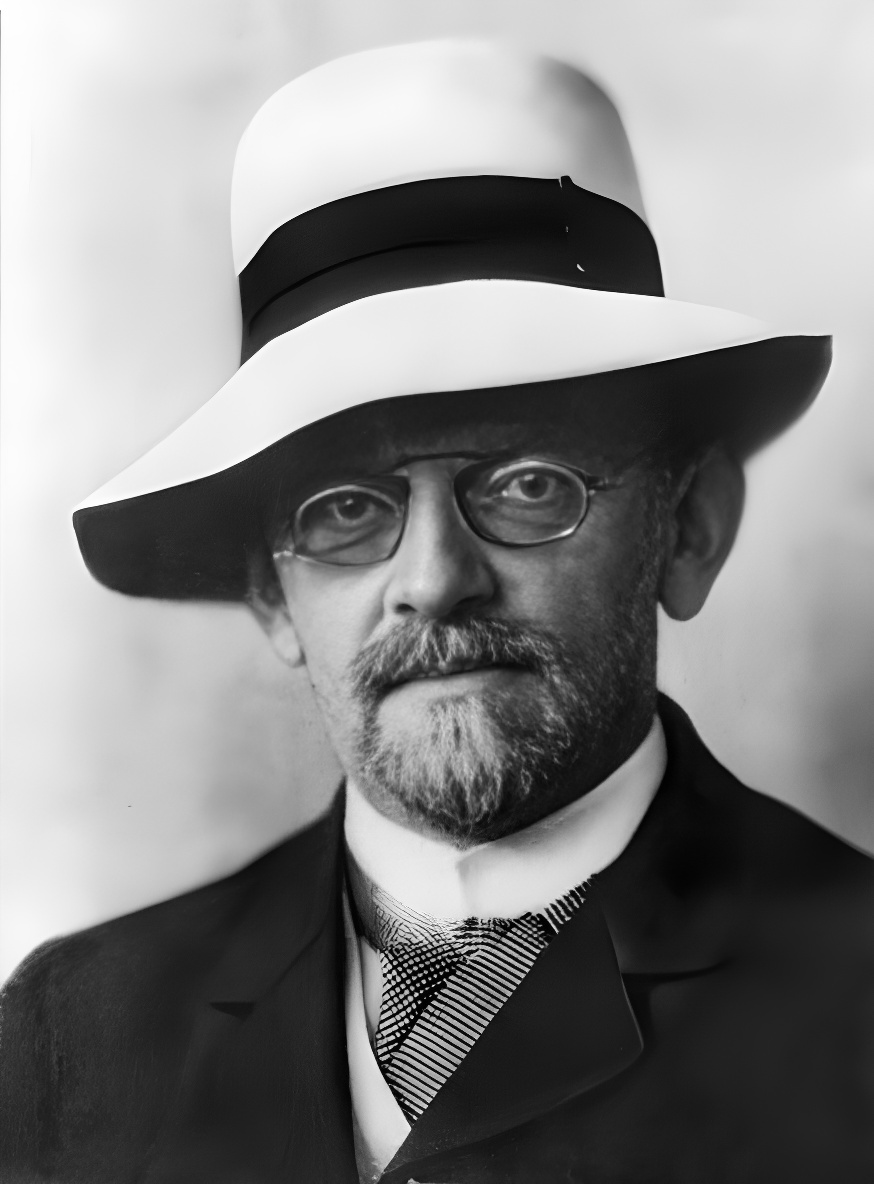
\includegraphics[width=4cm]{contents/images/hilbert}};
    \end{tikzpicture}
  \end{column}

\end{columns}

\end{frame}



\begin{frame}{Kolmogorov and Arnold's results}

\begin{columns}

  \begin{column}{7cm}
  \begin{itemize}
  \item Kolmogorov (1956): Every continuous multi-variable function
    can be expressed as the composition of a finite number of
    three-variable functions \vspace{0.3em}
  \item Arnold (1957): Only two-variable functions are really needed \vspace{0.3em}
  \item Kolmogorov (1957): Actually, the only two-variable function
    needed is addition \vspace{0.3em}
  \item This is a generalization of Hilbert's question, but the
    univariate functions are not necessarily algebraic
  \end{itemize}
  \end{column}

  \begin{column}{5cm}
    \begin{tikzpicture}
      \node (galois) {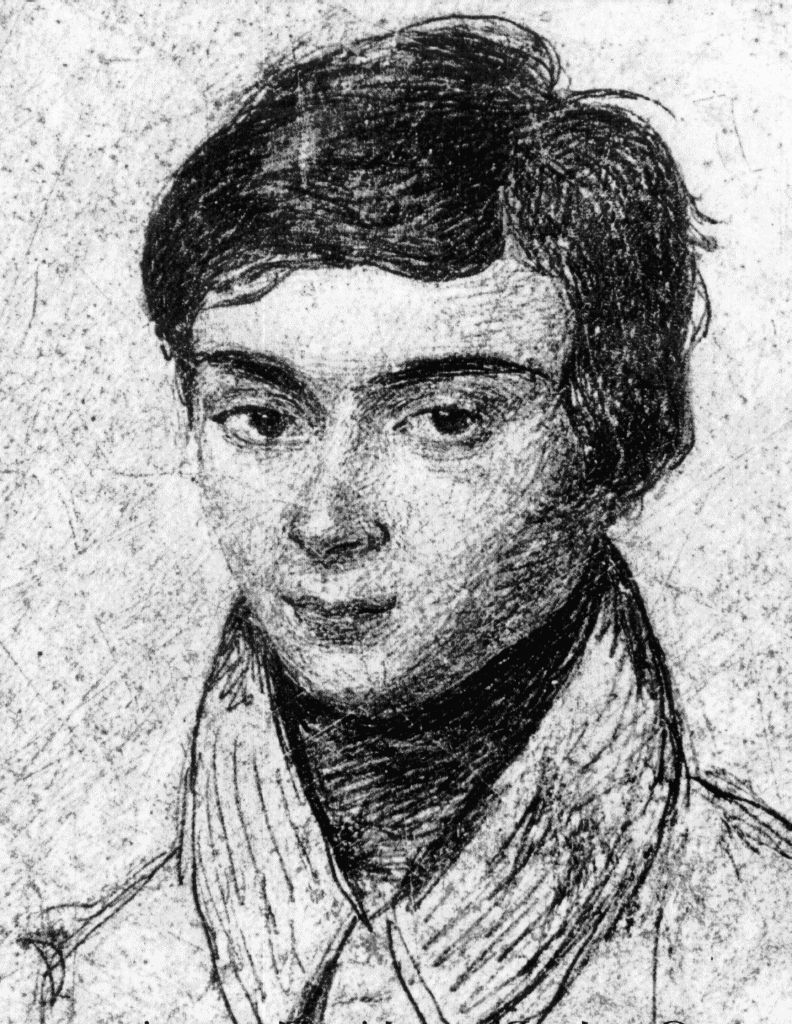
\includegraphics[width=2cm]{contents/images/galois}};
      \node (hilbert) at ([xshift=0.3cm] galois.south east)
            {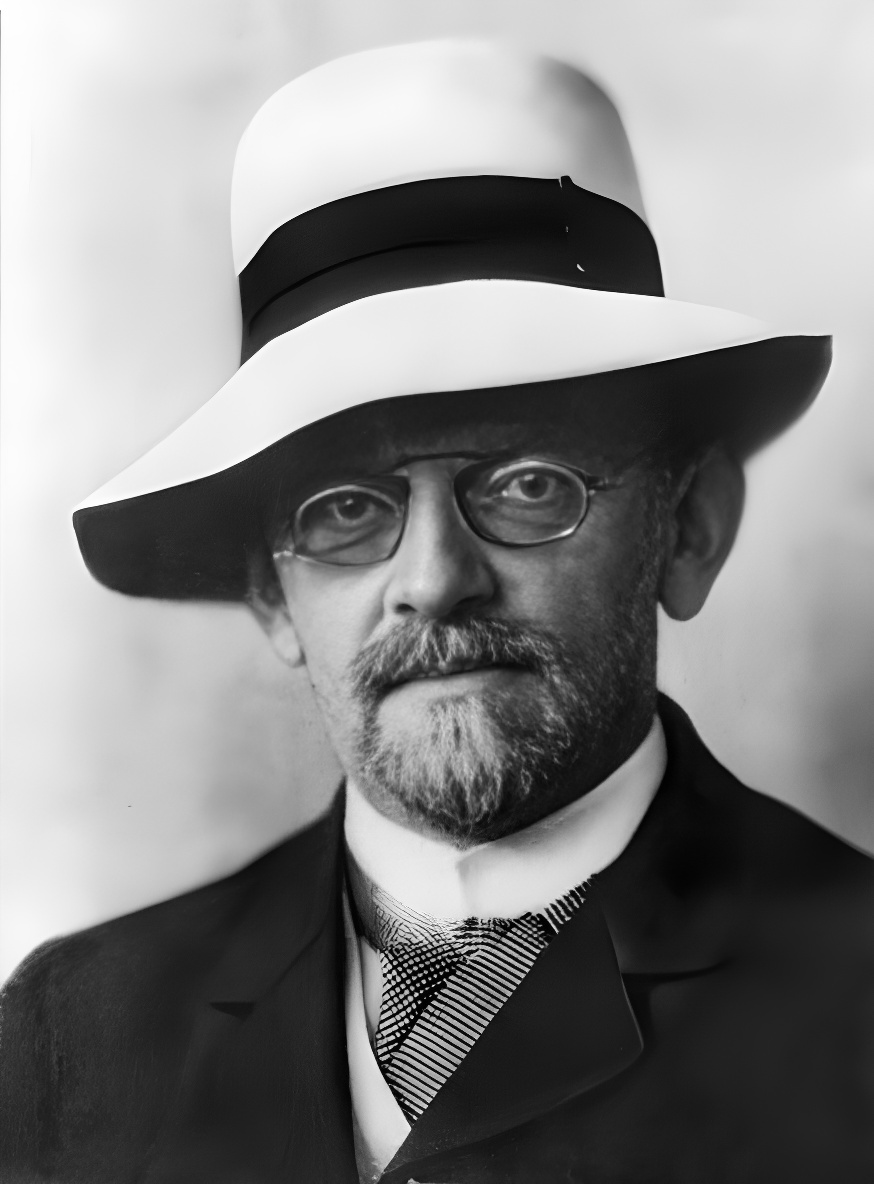
\includegraphics[width=3cm]{contents/images/hilbert}};
      \node (kolmogorov) at ([xshift=-1cm,yshift=0.5cm] hilbert.south west)
            {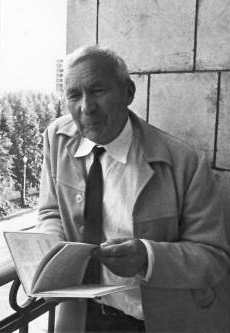
\includegraphics[width=3cm]{contents/images/kolmogorov}};
      \node (arnold) at ([xshift=-0.3cm,yshift=0.5cm] hilbert.south east)
            {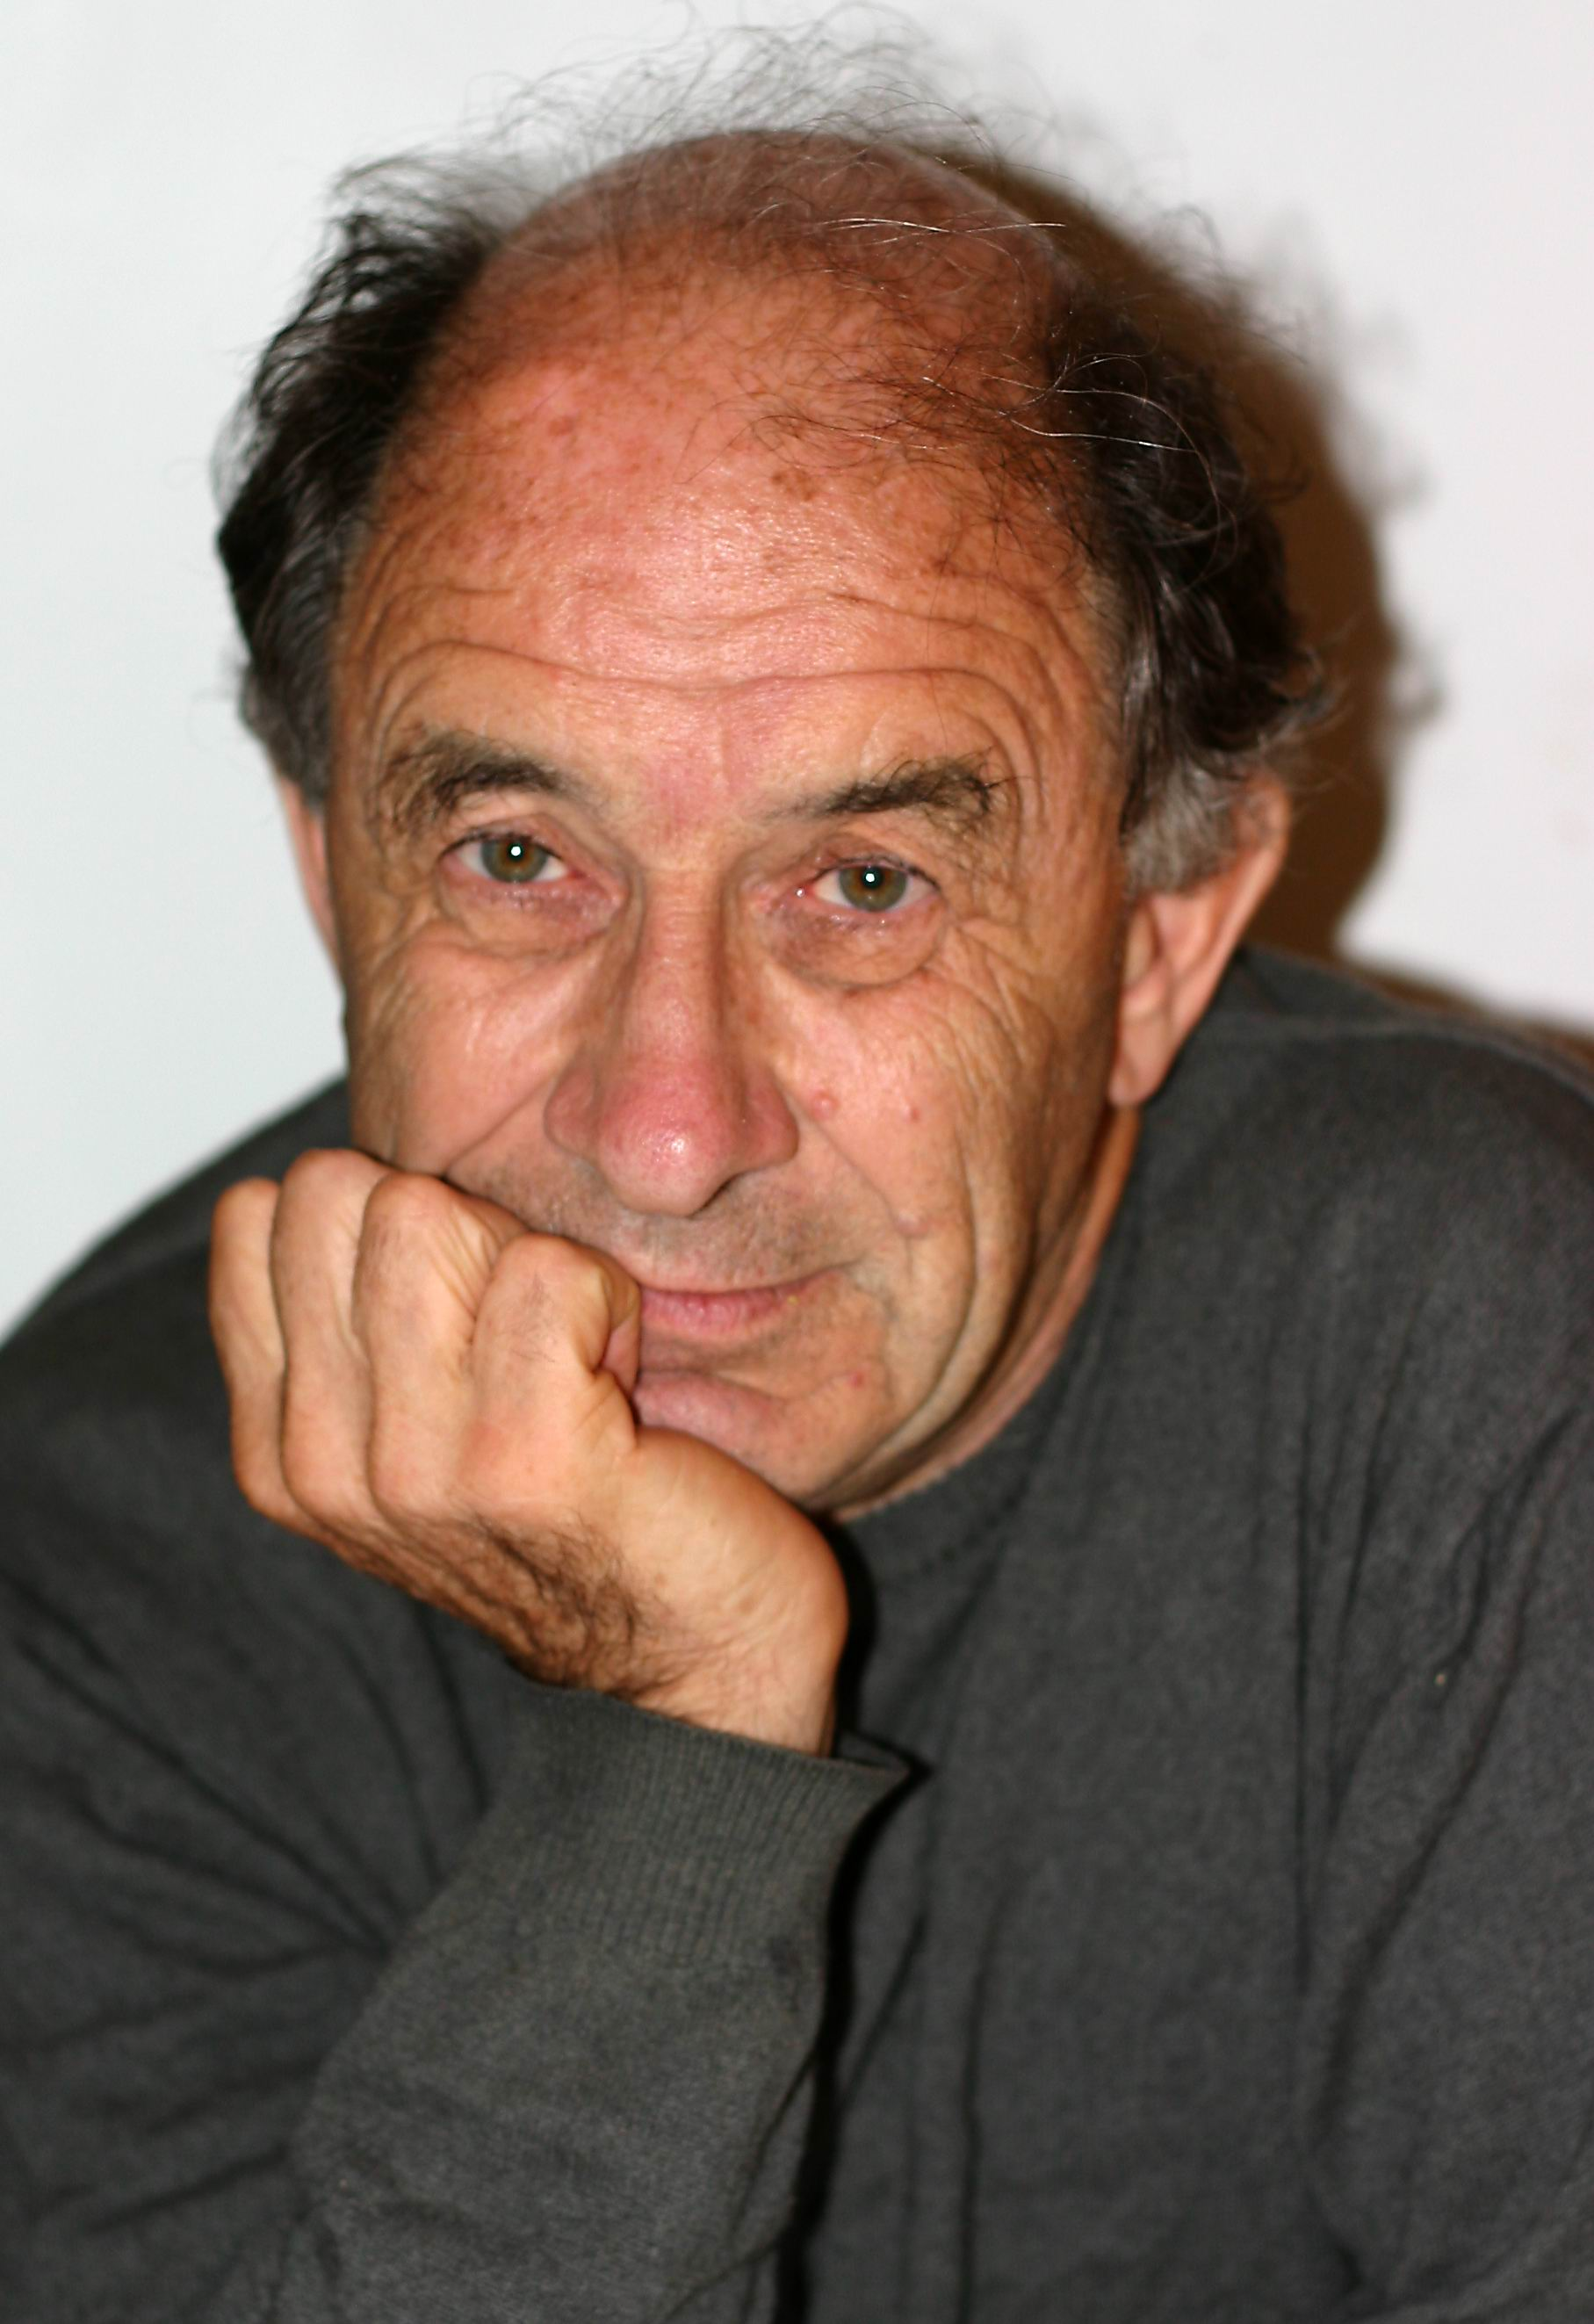
\includegraphics[width=3cm]{contents/images/arnold}};
    \end{tikzpicture}
  \end{column}

\end{columns}

\end{frame}



\begin{frame}{Kolmogorov-Arnold Representation Theorem}

\begin{columns}

  \begin{column}{6cm}
  \begin{itemize}
  \item Every multi-variate continuous function $f$ can be
    written using only univariate functions and addition:
    $$
    f(x_{i=1..n}) = \sum_{q=0}^{2n}\phi_q\left(\sum_{p=1}^n\psi_{q,p}(x_p)\right)
    $$
  \item In other words, addition is the only real multi-variate function,
    everything else is syntactic sugar
  \end{itemize}
  \end{column}

  \begin{column}{7cm}
  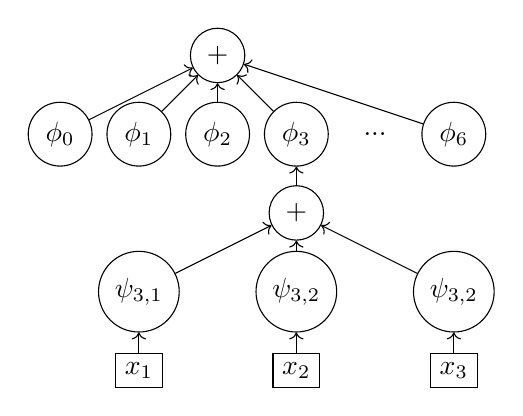
\begin{tikzpicture}
    \node[shape=circle,draw=black] (sum) at (0,0) {+};

    \node[shape=circle,draw=black] (F0) at (-2,-1) {$\phi_0$};
    \path [->] (F0) edge (sum);
    \node[shape=circle,draw=black] (F1) at (-1,-1) {$\phi_1$};
    \path [->] (F1) edge (sum);
    \node[shape=circle,draw=black] (F2) at (0,-1) {$\phi_2$};
    \path [->] (F2) edge (sum);
    \node[shape=circle,draw=black] (F3) at (1,-1) {$\phi_3$};
    \path [->] (F3) edge (sum);
    \node[shape=rectangle,draw=white] (dots) at (2,-1) {$...$};
    \node[shape=circle,draw=black] (F6) at (3,-1) {$\phi_6$};
    \path [->] (F6) edge (sum);

    \node[shape=circle,draw=black] (sum2) at (1,-2) {+};
    \path [->] (sum2) edge (F3);

    \node[shape=circle,draw=black] (f31) at (-1,-3) {$\psi_{3,1}$};
    \path [->] (f31) edge (sum2);
    \node[shape=circle,draw=black] (f32) at (1,-3) {$\psi_{3,2}$};
    \path [->] (f32) edge (sum2);
    \node[shape=circle,draw=black] (f33) at (3,-3) {$\psi_{3,2}$};
    \path [->] (f33) edge (sum2);

    \node[shape=rectangle,draw=black] (x1) at (-1,-4) {$x_1$};
    \path [->] (x1) edge (f31);
    \node[shape=rectangle,draw=black] (x2) at (1,-4) {$x_2$};
    \path [->] (x2) edge (f32);
    \node[shape=rectangle,draw=black] (x3) at (3,-4) {$x_3$};
    \path [->] (x3) edge (f33);

  \end{tikzpicture}
  \end{column}

\end{columns}

\end{frame}



\begin{frame}{Sprecher Formulation}

\begin{columns}

  \begin{column}{6cm}
  Sprecher (1972) gives an alternative formulation with a single function
  at the lower layer:
  $$
  f(x_{i=1..n}) = \sum_{q=0}^{2n}\phi_q\left(\sum_{p=1}^n\lambda^{p-1}\psi(x_p+q\cdot\epsilon)+q\right)
  $$
  where $\phi_q$ are continuous,
  $\psi$ is monotonically increasing and Lipschitz-1 continuous,
  $\lambda$ and $\psi$ depend only on $n$ and not on $f$,
  and $\epsilon$ is any non-zero constant
  \end{column}

  \begin{column}{7cm}
  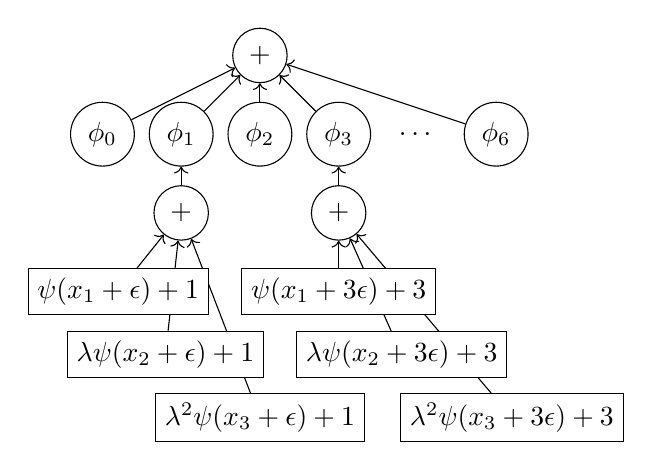
\begin{tikzpicture}
  \node[shape=circle,draw=black] (sum) at (0,0) {+};

  \node[shape=circle,draw=black] (F0) at (-2,-1) {$\phi_0$};
  \path [->] (F0) edge (sum);
  \node[shape=circle,draw=black] (F1) at (-1,-1) {$\phi_1$};
  \path [->] (F1) edge (sum);
  \node[shape=circle,draw=black] (F2) at (0,-1) {$\phi_2$};
  \path [->] (F2) edge (sum);
  \node[shape=circle,draw=black] (F3) at (1,-1) {$\phi_3$};
  \path [->] (F3) edge (sum);
  \node[shape=rectangle,draw=white] (dots) at (2,-1) {$\dots$};
  \node[shape=circle,draw=black] (F6) at (3,-1) {$\phi_6$};
  \path [->] (F6) edge (sum);

  \node[shape=circle,draw=black] (sum2) at (-1,-2) {+};
  \path [->] (sum2) edge (F1);

  \node[shape=rectangle,draw=black,fill=white] (l1) at (-1.8,-3) {$\psi(x_1+\epsilon)+1$};
  \node[shape=rectangle,draw=black,fill=white] (l2) at (-1.2,-3.8) {$\lambda\psi(x_2+\epsilon)+1$};
  \node[shape=rectangle,draw=black,fill=white] (l3) at (0,-4.6) {$\lambda^2\psi(x_3+\epsilon)+1$};
  \begin{scope}[on background layer]
    \path [->, behind path] (l1) edge (sum2);
    \path [->, behind path] (l2) edge (sum2);
    \path [->] (l3) edge (sum2);
  \end{scope}
    
  \node[shape=circle,draw=black] (sum4) at (1,-2) {+};
  \path [->] (sum4) edge (F3);

  \node[shape=rectangle,draw=black,fill=white] (l1) at (1,-3) {$\psi(x_1+3\epsilon)+3$};
  \node[shape=rectangle,draw=black,fill=white] (l2) at (1.8,-3.8) {$\lambda\psi(x_2+3\epsilon)+3$};
  \node[shape=rectangle,draw=black,fill=white] (l3) at (3.2,-4.6) {$\lambda^2\psi(x_3+3\epsilon)+3$};
  \begin{scope}[on background layer]
    \path [->] (l1) edge (sum4);
    \path [->] (l2) edge (sum4);
    \path [->] (l3) edge (sum4);
  \end{scope}

\end{tikzpicture}

  \end{column}

\end{columns}

\end{frame}



\begin{frame}{Some Thoughts and Intuitions}

\begin{itemize}
\item The theorem premises that $x_i$ are in the unit interval---this
  is needed for some of the constructions in the proof and is not a
  real restriction \vspace{0.5em}
\item The theorem proves the existence of the $\phi$ and $\psi$
  functions, does not tell you how to construct them \vspace{0.5em}
\item We know very little about $\phi$ (continuous) and slightly more
  (but still little) about $\psi$ (monotonic increasing and
  Lip-1 continuous) \vspace{0.5em}
\item It is unlikely that these functions can be defined by a
  neat-looking closed formula
\end{itemize}

\end{frame}



\begin{frame}{Some Thoughts and Intuitions}

\begin{columns}

  \begin{column}{6cm}
  \begin{itemize}
  \item Sprecher notes that he uses $\lambda^p$ but other non-linear
    sequences also work \vspace{0.5em}
  \item Feels like the $n$ values in the unit interval are
    \quotes{packed} into a single value in $\mathcal{R}$ and then
    \quotes{decoded} by the $\phi$ functions \vspace{0.3em}
    \begin{itemize}
    \item Note how $\lambda$ depends on $n$
    \end{itemize}
  \end{itemize}
  \end{column}

  \begin{column}{7cm}
  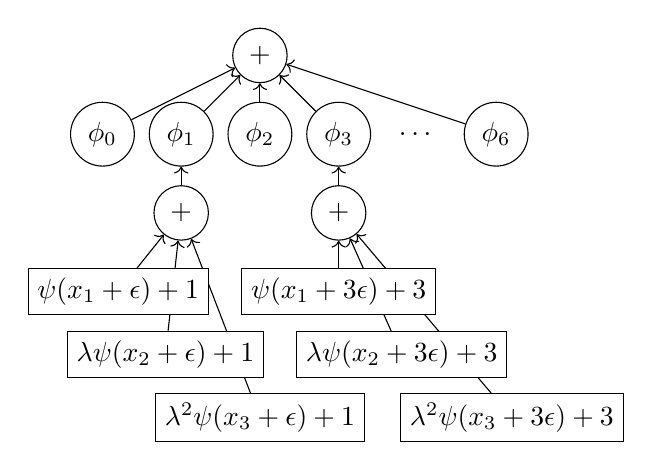
\begin{tikzpicture}
  \node[shape=circle,draw=black] (sum) at (0,0) {+};

  \node[shape=circle,draw=black] (F0) at (-2,-1) {$\phi_0$};
  \path [->] (F0) edge (sum);
  \node[shape=circle,draw=black] (F1) at (-1,-1) {$\phi_1$};
  \path [->] (F1) edge (sum);
  \node[shape=circle,draw=black] (F2) at (0,-1) {$\phi_2$};
  \path [->] (F2) edge (sum);
  \node[shape=circle,draw=black] (F3) at (1,-1) {$\phi_3$};
  \path [->] (F3) edge (sum);
  \node[shape=rectangle,draw=white] (dots) at (2,-1) {$\dots$};
  \node[shape=circle,draw=black] (F6) at (3,-1) {$\phi_6$};
  \path [->] (F6) edge (sum);

  \node[shape=circle,draw=black] (sum2) at (-1,-2) {+};
  \path [->] (sum2) edge (F1);

  \node[shape=rectangle,draw=black,fill=white] (l1) at (-1.8,-3) {$\psi(x_1+\epsilon)+1$};
  \node[shape=rectangle,draw=black,fill=white] (l2) at (-1.2,-3.8) {$\lambda\psi(x_2+\epsilon)+1$};
  \node[shape=rectangle,draw=black,fill=white] (l3) at (0,-4.6) {$\lambda^2\psi(x_3+\epsilon)+1$};
  \begin{scope}[on background layer]
    \path [->, behind path] (l1) edge (sum2);
    \path [->, behind path] (l2) edge (sum2);
    \path [->] (l3) edge (sum2);
  \end{scope}
    
  \node[shape=circle,draw=black] (sum4) at (1,-2) {+};
  \path [->] (sum4) edge (F3);

  \node[shape=rectangle,draw=black,fill=white] (l1) at (1,-3) {$\psi(x_1+3\epsilon)+3$};
  \node[shape=rectangle,draw=black,fill=white] (l2) at (1.8,-3.8) {$\lambda\psi(x_2+3\epsilon)+3$};
  \node[shape=rectangle,draw=black,fill=white] (l3) at (3.2,-4.6) {$\lambda^2\psi(x_3+3\epsilon)+3$};
  \begin{scope}[on background layer]
    \path [->] (l1) edge (sum4);
    \path [->] (l2) edge (sum4);
    \path [->] (l3) edge (sum4);
  \end{scope}

\end{tikzpicture}

  \end{column}

\end{columns}

\end{frame}



\begin{frame}{Some Thoughts and Intuitions}

\begin{columns}

  \begin{column}{6cm}
  \begin{itemize}
  \item $\psi$ has many `intervals' and translating by $q\cdot\epsilon$
    lands $x_i$ into the right interval
    \begin{itemize}
    \item hacks the multiple $\psi_i$ functions into one that
      behaves differently in each interval
    \end{itemize}
  \item The lower level `packs' the effect of~$f$ on~$x_i$ for
    different values of the other inputs $x_{j\neq i}$
  \item The upper level decodes to deliver the output
  \end{itemize}
  \end{column}

  \begin{column}{7cm}
  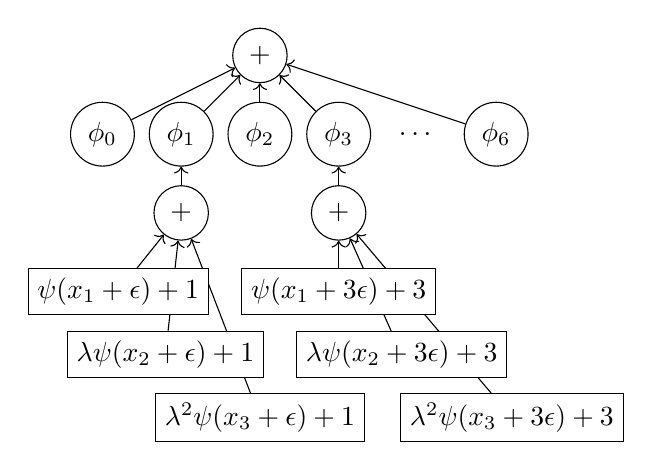
\begin{tikzpicture}
  \node[shape=circle,draw=black] (sum) at (0,0) {+};

  \node[shape=circle,draw=black] (F0) at (-2,-1) {$\phi_0$};
  \path [->] (F0) edge (sum);
  \node[shape=circle,draw=black] (F1) at (-1,-1) {$\phi_1$};
  \path [->] (F1) edge (sum);
  \node[shape=circle,draw=black] (F2) at (0,-1) {$\phi_2$};
  \path [->] (F2) edge (sum);
  \node[shape=circle,draw=black] (F3) at (1,-1) {$\phi_3$};
  \path [->] (F3) edge (sum);
  \node[shape=rectangle,draw=white] (dots) at (2,-1) {$\dots$};
  \node[shape=circle,draw=black] (F6) at (3,-1) {$\phi_6$};
  \path [->] (F6) edge (sum);

  \node[shape=circle,draw=black] (sum2) at (-1,-2) {+};
  \path [->] (sum2) edge (F1);

  \node[shape=rectangle,draw=black,fill=white] (l1) at (-1.8,-3) {$\psi(x_1+\epsilon)+1$};
  \node[shape=rectangle,draw=black,fill=white] (l2) at (-1.2,-3.8) {$\lambda\psi(x_2+\epsilon)+1$};
  \node[shape=rectangle,draw=black,fill=white] (l3) at (0,-4.6) {$\lambda^2\psi(x_3+\epsilon)+1$};
  \begin{scope}[on background layer]
    \path [->, behind path] (l1) edge (sum2);
    \path [->, behind path] (l2) edge (sum2);
    \path [->] (l3) edge (sum2);
  \end{scope}
    
  \node[shape=circle,draw=black] (sum4) at (1,-2) {+};
  \path [->] (sum4) edge (F3);

  \node[shape=rectangle,draw=black,fill=white] (l1) at (1,-3) {$\psi(x_1+3\epsilon)+3$};
  \node[shape=rectangle,draw=black,fill=white] (l2) at (1.8,-3.8) {$\lambda\psi(x_2+3\epsilon)+3$};
  \node[shape=rectangle,draw=black,fill=white] (l3) at (3.2,-4.6) {$\lambda^2\psi(x_3+3\epsilon)+3$};
  \begin{scope}[on background layer]
    \path [->] (l1) edge (sum4);
    \path [->] (l2) edge (sum4);
    \path [->] (l3) edge (sum4);
  \end{scope}

\end{tikzpicture}

  \end{column}

\end{columns}

\end{frame}


\begin{frame}{Proof Sketch}

The actual proof is between $E^n$ and $E^{n-1}$, which gives inductively
that a function in $E^n$ can be represented with functions in $E$.

To allow for nice figures, we will show that for any $f:E^2\rightarrow\mathcal{R}$
there are $\phi_{0..4}:\mathcal{R}\rightarrow\mathcal{R}$
and $\psi_{0..4,1..2}:E\rightarrow\mathcal{R}$ such that:
$$
f(x_1,x_2)=\sum_{q=0}^4\phi_q\left(\psi_{q,1}\left(x_1\right)+\psi_{q,2}\left(x_2\right)\right)
$$

The proof proceeds in three steps:
%
\begin{itemize}
\item Cover the unit square
\item Construct the inner functions $\psi$
\item Construct the outer functions $\phi$
\end{itemize}
\end{frame}



\begin{frame}{Proof Sketch Step 1: Cover the unit square}

For any integer $k>0$, we can construct $k$ non-overlapping intervals
in $E$ with length less than $1/k$
As $k>0$ gets larger, the length of each interval gets smaller; at the
limit the length of each interval will approach zero.

\vskip 1em

Fix a value for $k$.

\vskip 1em

Let $A_{k,1}$ be the union of such intervals for $p=1$ (i.e., for the
first input of $f$).

\vskip 1em

We repeat the process to make one such union $A_{k,1}^q$ for each
value of $q = 0..2n$. All $A_{k,1}^q$ are one
\emph{family} and all $A_{k,2}^q$ are another family. There are
$n=2$ families.

\end{frame}



\begin{frame}{Proof Sketch Step 1: Cover the unit square}

\textcolor{blue!50!black}{Every $x\in E$ is contained in no less than $2n$ (here, 4) members of the family}

\vskip 1 em

The families can always be constructed so that the gaps of their
members do not intersect:

\vskip 1 em

\begin{tabular}{lccccccccccccccc}
\hline
$A_{k,1}^0$ & x & x & x & x & x & x &   & x & x & x & x & x & x &   & x \\ 
\hline
$A_{k,1}^1$ &   & x & x & x & x & x & x &   & x & x & x & x & x & x &   \\
\hline
$A_{k,1}^2$ & x &   & x & x & x & x & x & x &   & x & x & x & x & x & x \\
\hline
$A_{k,1}^3$ & x & x &   & x & x & x & x & x & x &   & x & x & x & x & x \\
\hline
$A_{k,1}^4$ & x & x & x &   & x & x & x & x & x & x &   & x & x & x & x \\
\hline
\end{tabular}  
\vskip 1 em

so that any point in $E$ will be contained in at most one gap.

\end{frame}



\begin{frame}{Proof Sketch Step 1: Cover the unit square}

\begin{itemize}

\item Replicate the family $A_{k,1}^q$ into $A_{k,2}^q$ \vspace{0.5em}

\item For each $q$, constuct $S_k^q$, the union of the non-overlapping
  squares $A_{k,1}^q \times A_{k,2}^q$ \vspace{0.5em}

\item Any point in $E^2$ will be contained in at most one gap in each
  dimention, so will be contained in at least $2n+1-n = n+1$
  intervals \vspace{0.5em}

\end{itemize}
\vskip 1em

\textcolor{blue!50!black}{%
  The system of all rectangles $S_k^q, q=0..2n$ covers the unit square
  $E^2$ so that every point in $E^2$ is covered at least $n+1$ times.
}

\end{frame}



\begin{frame}{Proof Sketch Step 2: Construct the inner functions}

\begin{columns}

  \begin{column}{7cm}

  For given $k,q$, it is always possible to construct a series of
  constants $\lambda_i$ such that:

  $$
  \lambda_i < \lambda_{i+1} \leq \lambda_i + \frac{1}{2^k}
  $$

  and a function $\psi_1$ mapping inputs from the
  $A_{k,1}^q$ intervals to the corresponding $\lambda$ intervals.

  \vskip 1em

  Any continuous function will do, but let's say its a step function
  with linear connections across gaps, so that it's continuous and
  monotonic increasing.

  \end{column}

  \begin{column}{6.5cm}
  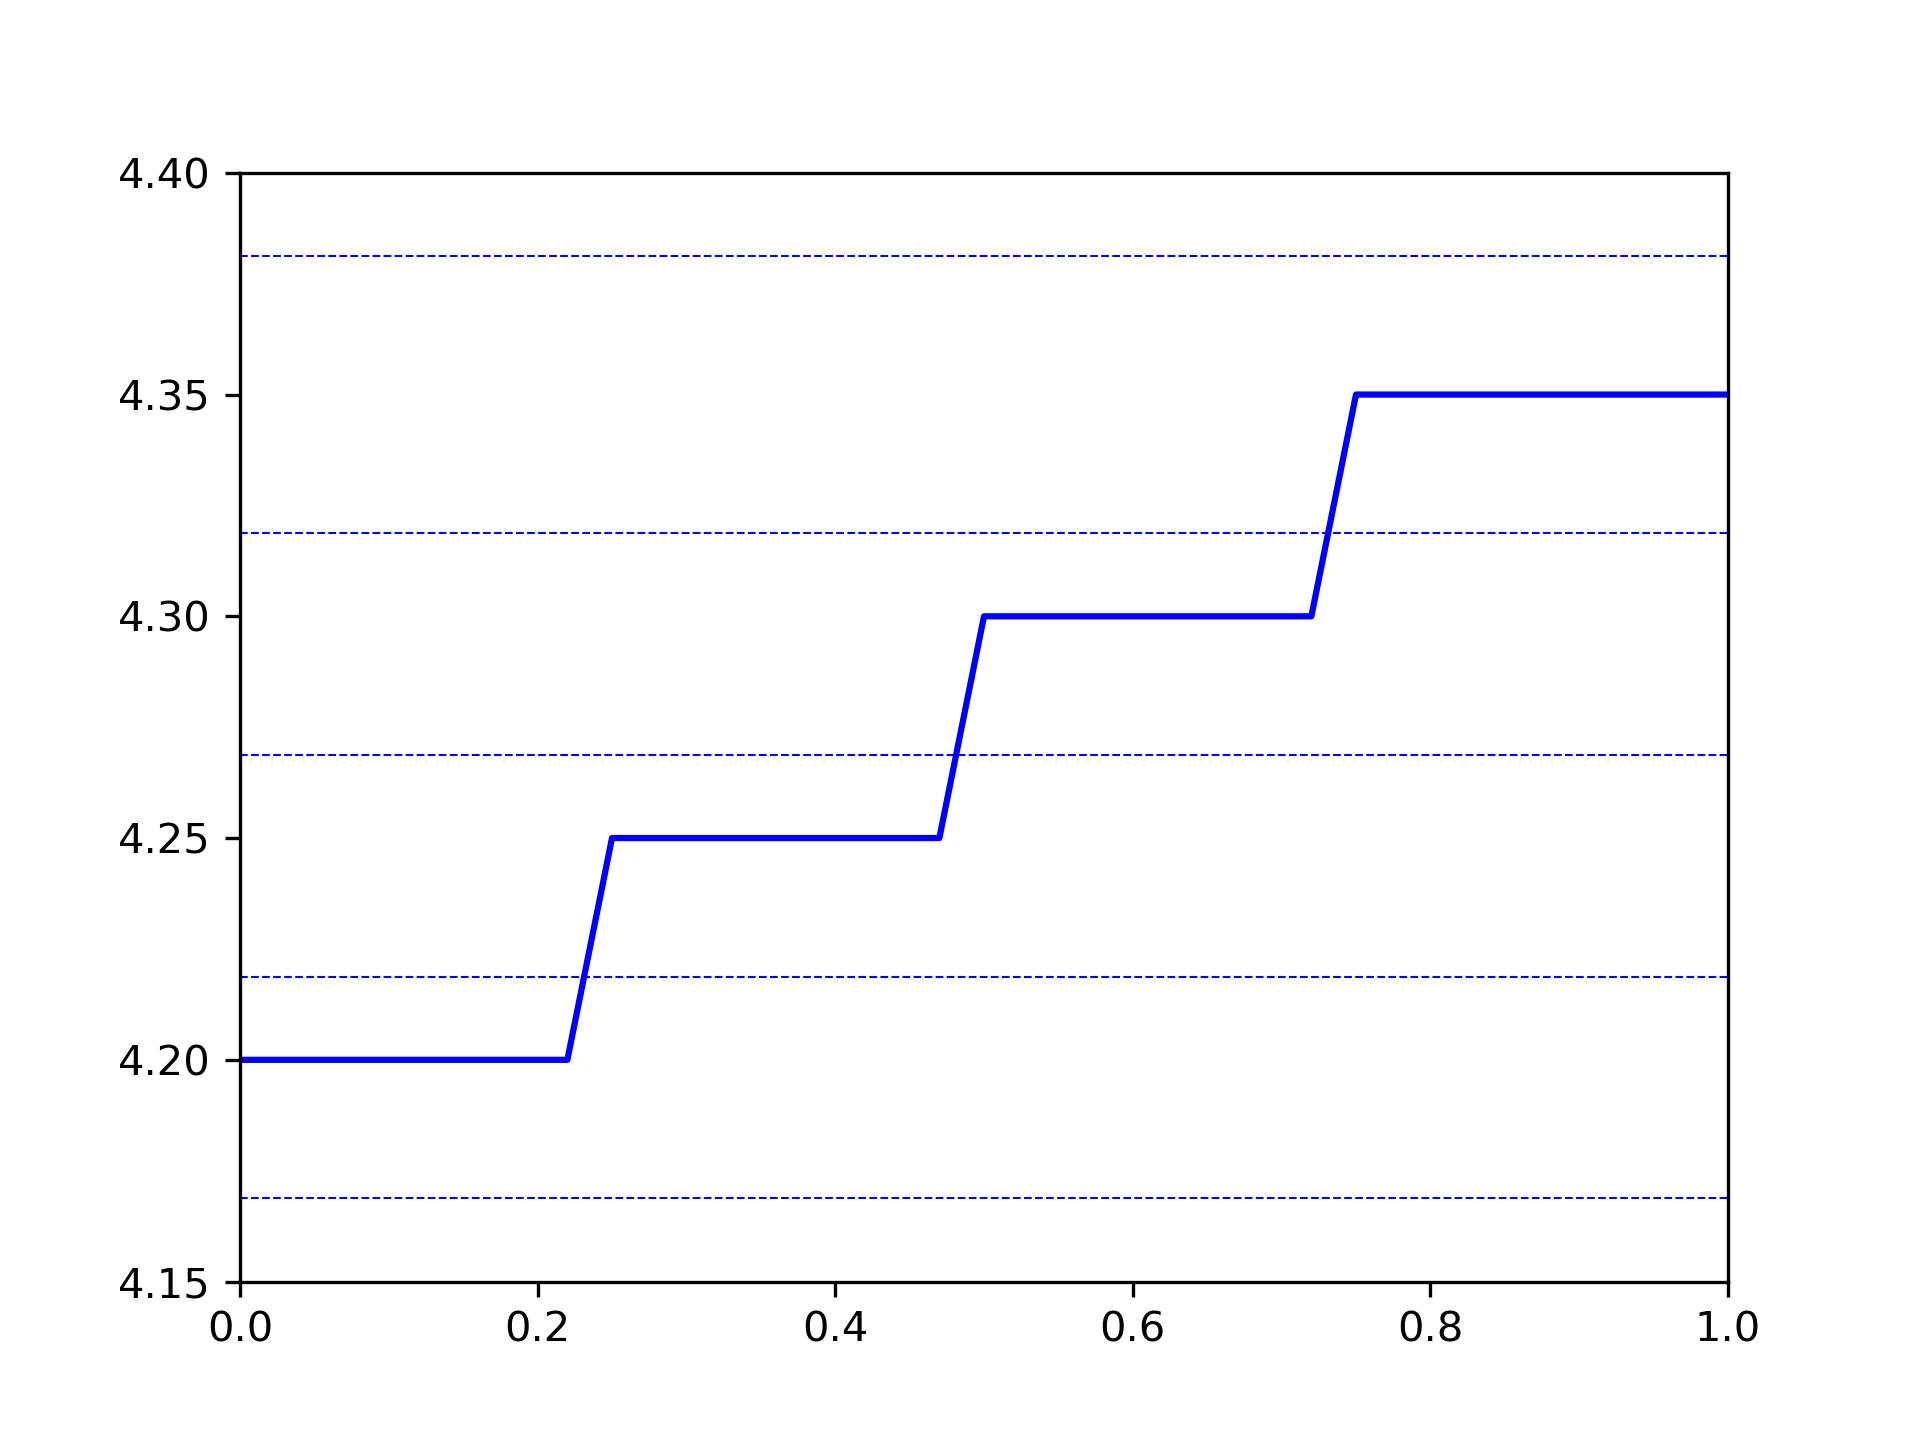
\includegraphics[width=6cm]{contents/images/kat_psi1}

  For $k=4$, four non-overlapping intervals and
  the corresponding `lanes' defined by the $\lambda$ series.
  \end{column}

\end{columns}

\end{frame}



\begin{frame}{Proof Sketch Step 2: Construct the inner functions}

Construct a similar series $\mu_i$ for the second dimension.
Then:
$$
\lambda_i+\mu_i < \lambda_{i+1}+\mu_{i+1} \leq \lambda_i + \mu_i + 2\frac{1}{2^k}
$$
so an $\epsilon_k < 2^{-k}$ can be found such that the closed intervals
$\left[ \lambda_i+\mu_i , \lambda_i+\mu_i+2\epsilon_k \right]$
do not intersect.

\vskip 1em

Since they do not intersect, we can apply the same logic as before to
construct two functions $\psi_1,\psi_2$
such that their addition maps elements from the $S_k$ squares
we constructed before, to values within these intervals:

$$
\mbox{For each } x_1,x_2\in S_k^q,
\psi_1(x_1)+\psi_2(x_2) \in \left[ \lambda_i+\mu_i , \lambda_i+\mu_i+2\epsilon_k\right]
$$

\end{frame}



\begin{frame}{Proof Sketch Step 2: Construct the inner functions}

\begin{columns}

  \begin{column}{7cm}
  There are many solutions, but Sprecher's (1972) formulation gives us
  something we can visualize:
  \vskip 1em
  A grid of non-overlapping \quotes{platforms}, linearly connected at the
  gaps, all having different $z$, so that each $z$ maps to exactly
  one $S_k$ or to a gap.
  \end{column}

  \begin{column}{6.5cm}
  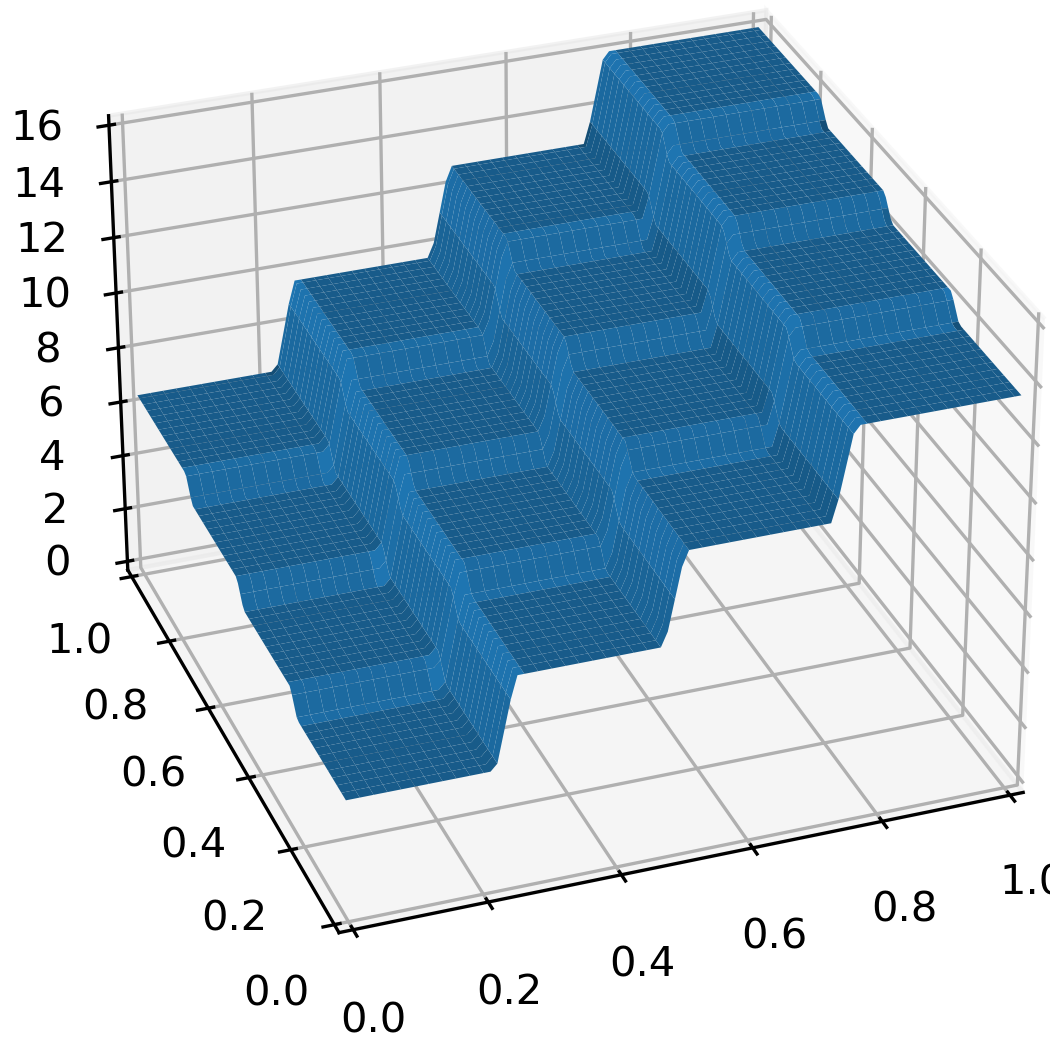
\includegraphics[width=6cm]{contents/images/kat_psi3}
  \end{column}

\end{columns}

\end{frame}



\begin{frame}{Proof Sketch Step 2: Construct the inner functions}

Reminder from Step 1:
\vspace{0.5em}
\begin{itemize}
\item For each $q=0..2n$, we constucted a family of non-overlapping
  squares $S_k^q$
\item Every point in $E^2$ is covered by at least $n+1$ squares
\end{itemize}

\vskip 1em

So we repeat all the above for all $q$ to create $2n+1$ different
$n$-tuples of $\psi$ functions.

\vskip 1em

\begin{itemize}
\item For each $q$, we have created a mapping from some values of
  $\psi_1(x_1)+\psi_2(x_2)$ to a $S_k^q$. The rest of the possible values
  of $\psi_1(x_1)+\psi_2(x_2)$ might be over a gap, but:
\item For each $x_1,x_2\in E^2$, at least $n+1$ of the $q$ families are not
  gaps
\end{itemize}

\end{frame}



\begin{frame}{Proof Sketch Step 3: Construct the outer functions}

All the pieces are now in place:
\vspace{0.5em}
\begin{itemize}
\item We have an `index' from $\psi_1(x_1)+\psi_2(x_2)$ to squares
  restricting the possible values of $x_1,x_2$. The size of the
  squares gets smaller as $k$ gets larger. \vspace{0.4em}
\item We can construct a function $f_k$ that simply `memorizes' how to
  approximate the value of the original $f$ from the sum of $\phi_p$ \vspace{0.3em}
  \begin{itemize}
  \item all pairs in the unit square are covered
  \item $f_k$ knows the neighbourhood of the $x_1,x_2$ values despite the fact
    that only sees sums
  \item $f_k$ can estimate $f$ with some error bounded by an
    expression denominated by $k$
  \end{itemize} \vspace{0.4em}
\item At the limit, there is no error
\end{itemize}

\vskip 0.8em

\textcolor{blue!50!black}{%
  Unlike the $\psi$ functions, we have no intuitions whatsoever
  about what the $\phi$ functions look like or how to construct them.
}

\end{frame}



\begin{frame}{Some More Thoughts}

There are many ways to pack two real numbers into one and then define
the function that unpacks the original numbers and applies $f$.
Here is one packing schema:

\vskip 1em

\begin{center}

  \begin{tabular}{l}
    0.42 \\
    0.31415926$\dots$ \\
    \hline
    0.4321040105090206$\dots$ \\
  \end{tabular}
  \end{center}

\vskip 0.5em

The Kolmogorov-Arnold therom tells us that it is possible to find a
\textbf{continuous} function that does the same
\vspace{0.5em}
\begin{itemize}
\item 'Continuous' sounds like a positive quality, but many
  `pathological' functions are nominally continuous
\item Under this light, we consider the claim that addition is the
  only multi-variate function strictly speaking valid, but over-hyped
\end{itemize}

\end{frame}



\begin{frame}{Some More Thoughts}

Kudos to Kolmogorov and Arnold for:
\vspace{0.5em}
\begin{itemize}
\item Anticipating modern ML: As long as it fits the data, it doesn't
  matter if the model captures the actual structures that generate the data \vspace{0.5em}
\item Anticipating modern ML II: In the executive summary, over-hype
  the significance of the result \vspace{0.5em}
\item Anticipating that multiple arguments can be passed as one complex
  \strong{record} a couple of years before COBOL \vspace{0.5em}
\item Making people reconsider the definition of \strong{function complexity}
\end{itemize}

\end{frame}



\begin{frame}{Post-KART}

\begin{itemize}
\item Hilbert's intuition about not being able to represent more
  complex functions by algebraically combining simpler functions remains valid:
  \begin{itemize}
  \item It obviously remains open for algebraic functions
  \item Its essense holds for any function, except that the K-A
    Representation Theorem proves that using the number of arguments
    to define complexity is wrong
  \item Vitushkin~(2004) gives a compelling argument
  \end{itemize}
\vspace{0.5em}
\item Hecht-Nielsen (1987) notes the similarity between Sprecher's
  formulation and NNs and speculates that NN training can be used to
  construct $\phi$, but Girosi \& Poggio (1989) point out that we know
  $\phi$ are not smooth (Vitushkin \& Henkin, 1967) and cannot be
  learnt.
\vspace{0.5em}
\item Schmidt-Hieber (2021) gives a good overview of the ways the KART
  has interacted with the ML community.
  
\end{itemize}

\end{frame}



\section{Kolmogorov-Arnold Networks}
{
  \setbeamertemplate{headline}{}
  \begin{frame}
    \sectionpage%
  \end{frame}
}


\begin{frame}{Neural Networks are Function Approximators}

\begin{itemize}
    \item MLPs are inspired by the \strong{Universal Approximation Theorem} \vspace{0.5em}
    \begin{itemize}
        \item Leshno et al. (1993):
        \textit{A standard multilayer FNN can approximate any continuous function to any degree of accuracy iff
        the network’s activation functions are not polynomial}
    \end{itemize}
    \vspace{1em}
    \item Can we be inspired by \strong{KART}?
\end{itemize}

\end{frame}

\begin{frame}{Neural Networks are Function Approximators}

\begin{itemize}
    \item Can we be inspired by \strong{KART}?
    \begin{itemize}
        \item KART claims that learning a high-dimensional function reduces to learning a polynomial number of 1D functions then, why \textbf{inspired}? \dots
        \item \dots these 1D functions can be non-smooth (aka \textit{not learnable!})
        \item \dots using only 2-layer nonlinearities and $2n + 1$ terms in the hidden layer is pretty restrictive
    \end{itemize}
    \vspace{1em}
    \item \textit{But},
    \begin{itemize}
        \item We can argue that most ML-concerning functions are smooth, and
        \item We can just stack $\phi$ layers and pray
    \end{itemize}
    \vspace{1em}
    \item So, we are no longer using KA(R)T but moving towards a KA(A)T
    \vspace{1em}
    \item This is how \strong{Kolmogorov-Arnold Networks (KANs)} are born (Ziming Liu et al., 2024)
\end{itemize}

\end{frame}

\begin{frame}{Architecture: High Level}
  \begin{columns}
      \begin{column}{8.5cm}
      \begin{itemize}
        \item \textit{Inspiration:} KART
        $$f(x_1,\dots,x_n) = \sum_{q=0}^{2n}\phi_q\left(\sum_{p=1}^n\psi_{q,p}(x_p)\right)$$
        \item We just need to learn the univariate functions $\psi$ and $\phi$ and perform addition
        \vspace{0.5em}
        \item \strong{($\rightarrow$)} A shallow KAN representing the above equation, with $n=2$ input variables $x_p$,\\ $2n+1=5$ $\phi_{\text{s}}$ and  $f(x_1,x_2)$ as the output
        \vspace{0.5em}
        \item Learnable activation functions are positioned on edges and summation is performed on nodes
      \end{itemize}
    \end{column}

    \begin{column}{5cm}
      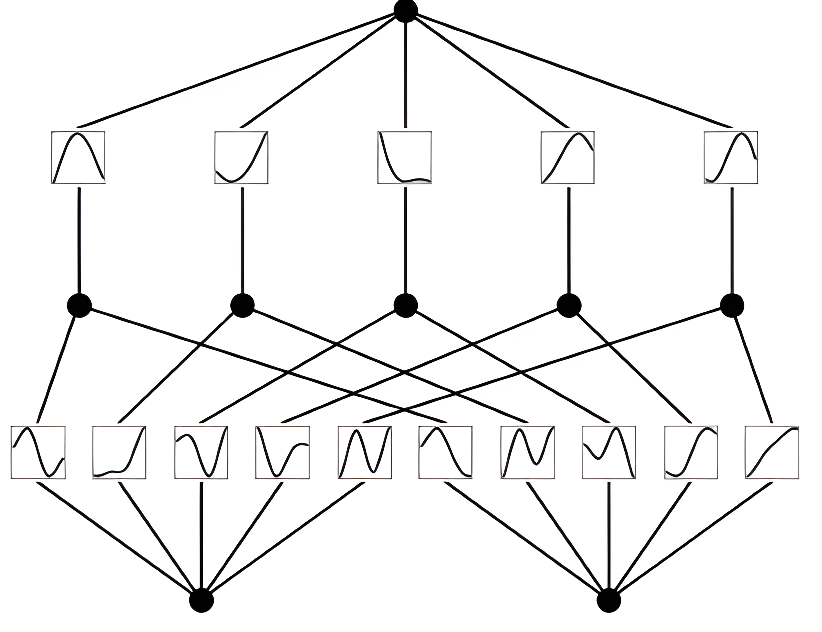
\includegraphics[width=5cm]{contents/images/KAN_arch_simple}
    \end{column}
  \end{columns}
\end{frame}

\begin{frame}{Architecture: Comparison with MLP}
    \strong{Shallow Formula} \vspace{0.3em}
    \begin{itemize}
        \item Though KART ensures exact representation and UAT guarantees approximation, relaxing KART's assumptions positions both as function approximators \vspace{0.5em}
        \item UAT lacks guarantees on shallow MLP size, and KART provides no method to compute the relative functions \vspace{0.5em}
        %A set G\subseteq F of functions is called dense in a function space F, if it can approximate any function f\in F to an arbitrary degree of accuracy.
        %In other words, given any real function f\in F and ε>0, there is a real function g\in G for which |g(x) - f(x)|<ε
        \item MLP uses fixed activations on nodes and learnable weights on edges, while KAN employs fixed learnable functions on edges and summation on nodes \vspace{0.5em}
    \end{itemize}
\end{frame}

\begin{frame}{Architecture: Comparison with MLP}
    \strong{Deep Formula} \vspace{0.3em}
    \begin{itemize}
        \item Shifting to deep formula to avoid UAT's and KART's restrictions \vspace{0.3em}
        \item KAN shifts non-linearity computation to the composition of $\phi_{\text{s}}$ rather than the
        weights and activation functions in MLPs \vspace{0.3em}
        \item KAN defines a \textit{KAN layer} with $n_{\text{in}}$-D inputs and $n_{\text{out}}$-D
        outputs as a matrix of 1D functions, stacking these layers (note how we are drifting further away from KART)\vspace{0.3em}
        \item So, the dimensions of the KAN are \textit{not} restricted to $[n, 2n+1, 1]$
    \end{itemize}
\end{frame}

\begin{frame}{Architecture: Lower Level}
    \begin{itemize}
        \item The learnable univariate functions are parametrized as a \textbf{B-spline (basis spline) curves} with learnable coefficients of local B-splines \vspace{0.3em}
        \item Splines are a transformation that maps control points to a smooth curve, aiming to generally follow the shape of these points \vspace{0.3em}
        \item Let us present the B-splines in depth \vspace{0.3em}
    \end{itemize}
\end{frame}

\begin{frame}{B\'ezier curves: Linear}
        To create a path between 2 points $P_0$ and $P_1$, we perform \textbf{linear interpolation} :
         \vspace{1em}
        $$P(t) = (1-t)P_0 + tP_1$$
        \vspace{0.5em}
        \begin{center}
            
\includegraphics[width=5cm]{contents/images/linear_interpolation_1}
        \end{center}
\end{frame}

\begin{frame}{B\'ezier curves: Quadratic}
    \begin{itemize}
        \item If we add a third point $P_2$, then we have two lines connecting them and we can perform linear interpolation to them as well
        \vspace{1em}
        \begin{center}
            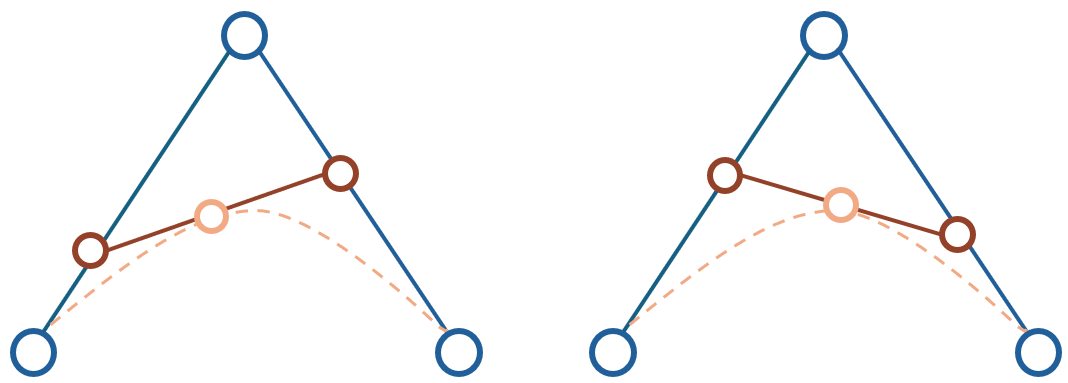
\includegraphics[width=10cm]{contents/images/quadratic_bezier_3}
        \end{center}\vspace{1em}
        \item This curve is called a \textbf{quadratic} \strong{B\'ezier curve}
    \end{itemize}
\end{frame}

\begin{frame}{B\'ezier curves: Cubic and higher}
    \begin{itemize}
        \item In the same spirit, we can define the \textbf{cubic B\'ezier curve} (and any other degree, respectively)
        \vspace{1em}
        \begin{center}
            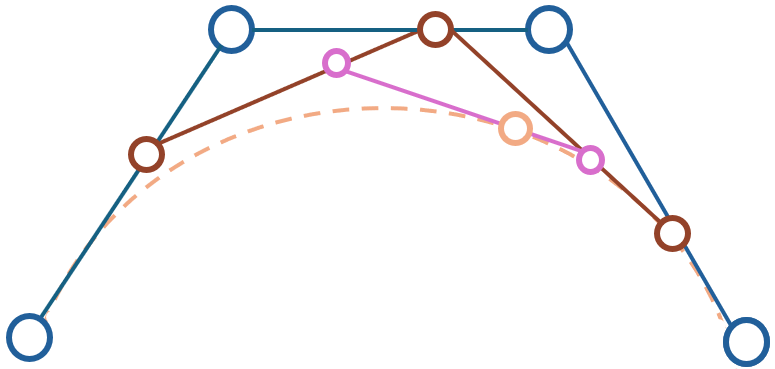
\includegraphics[width=6cm]{contents/images/cubic_bezier}
        \end{center} \vspace{0.8em}
        \item We call the points \textbf{control points}, since the control the curvature
    \end{itemize}
\end{frame}

\begin{frame}{B\'ezier curves: Algorithms}
    \begin{itemize}
        \item This repeated linear interpolation is called the \textbf{de Casteljau} algorithm \vspace{0.2em}
        \item A less expensive method for computing B\'ezier curves involves solving the \textbf{Bernstein polynomials} which are the linear interpolation equations expressed wrt the points
    \end{itemize}
    \begin{columns}
            \begin{column}{5cm}
                 \begin{center}
                    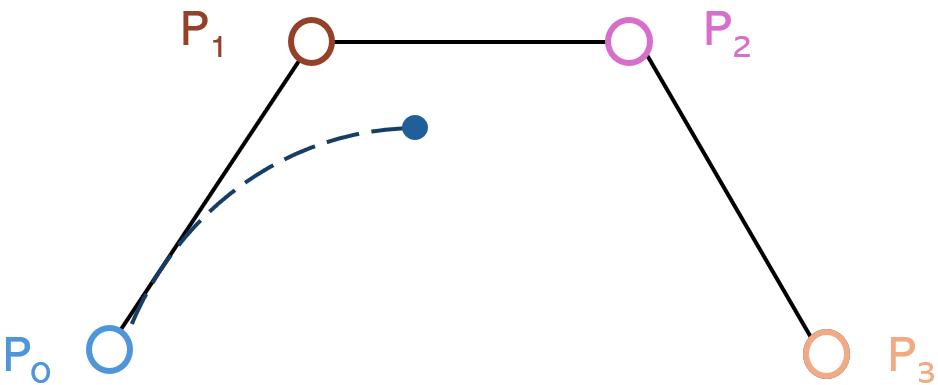
\includegraphics[width=5cm]{contents/images/cubic_bernstein}
                \end{center}
            \end{column}
            \begin{column}{2.5cm}
                \begin{center}
                 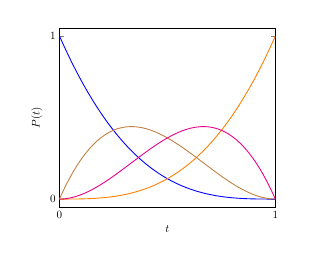
\begin{tikzpicture}[scale=0.4]
                    \begin{axis}[
                        xlabel={$t$},
                        ylabel={$P(t)$},
                        xmin=0, xmax=1,
                        ymin=-0.05, ymax=1.05,
                        xtick={0,1},
                        ytick={0,1},
                        xtick pos=both,
                        ytick pos=both,
                        grid=none,
                        %legend style={at={(1.05,1)},anchor=north west},
                        %legend cell align={left}
                    ]
                        \addplot[domain=0:1, samples=100, thick, color=blue]
                            {-x^3 + 3*x^2 - 3*x + 1};
                        %\addlegendentry{$-t^3 + 3t^2 - 3t + 1$}

                        \addplot[domain=0:1, samples=100, thick, color=orange]
                            {x^3};
                        %\addlegendentry{$t^3$}

                        \addplot[domain=0:1, samples=100, thick, color=brown]
                            {3*x^3 - 6*x^2 + 3*x};
                        %\addlegendentry{$3t^3 - 6t^2 + 3t$}

                        \addplot[domain=0:1, samples=100, thick, color=magenta]
                            {-3*x^3 + 3*x^2};
                        %\addlegendentry{$-3t^3 + 3t^2$}
                    \end{axis}
                \end{tikzpicture}
                \end{center}
            \end{column}
            \begin{column}{4.5cm}
              \scalebox{0.8}{%
                $\begin{aligned}
                  P(t) = \quad
                  & \textcolor{blue!90!black}{P_0} \cdot (-t^3 + 3t^2 - 3t + 1) +\\
                  & \textcolor{brown!70!black}{P_1} \cdot (3t^3 - 6t^2 + 3t) +\\
                  & \textcolor{magenta!80!black}{P_2}\cdot (-3t^3 + 3t^2) +\\
                  & \textcolor{orange!80!black}{P_3} \cdot (t^3)
                \end{aligned}$
              }
            \end{column}
    \end{columns}
    \begin{itemize}
        \vspace{0.2em}
        \item If we plot the factors of these polynomials we get a visualization of the influences of the control points (cf. right Illustration)
    \end{itemize}
\end{frame}

\begin{frame}{B\'ezier curves: (lack of) local control}
    \begin{itemize}
        \item One main downside of B\'ezier curves is the lack of local control
        \item This means that by changing \textbf{only one} control point, the curve can change drastically
        \item \strong{Pay attention because we will need this later on!}
    \end{itemize}
    \begin{columns}
        \begin{column}{5cm}
            \begin{figure}[h!]
                \centering
                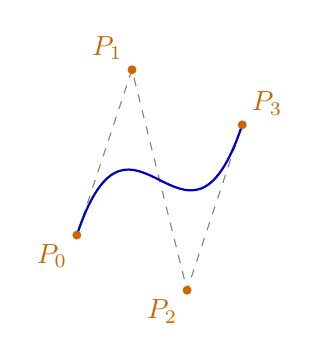
\begin{tikzpicture}[scale=0.7]
                    \coordinate (P0) at (0, 0);
                    \coordinate (P1) at (1, 3);
                    \coordinate (P2) at (2, -1);
                    \coordinate (P3) at (3, 2);

                    \draw[gray, dashed] (P0) -- (P1) -- (P2) -- (P3);
                    \draw[thick, blue!80!black] (P0) .. controls (P1) and (P2) .. (P3);

                    \filldraw[orange!80!black] (P0) circle (2pt) node[below left] {$P_0$};
                    \filldraw[orange!80!black] (P1) circle (2pt) node[above left] {$P_1$};
                    \filldraw[orange!80!black] (P2) circle (2pt) node[below left] {$P_2$};
                    \filldraw[orange!80!black] (P3) circle (2pt) node[above right] {$P_3$};
                \end{tikzpicture}
            \end{figure}
        \end{column}

        \begin{column}{5cm}
             \begin{figure}[h!]
                \centering
                 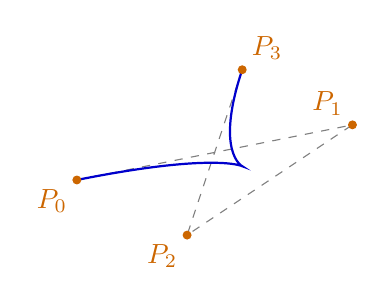
\begin{tikzpicture}[scale=0.7]
                    \coordinate (P0) at (0, 0);
                    \coordinate (P1) at (5, 1);
                    \coordinate (P2) at (2, -1);
                    \coordinate (P3) at (3, 2);

                    \draw[gray, dashed] (P0) -- (P1) -- (P2) -- (P3);

                    \draw[thick, blue!80!black] (P0) .. controls (P1) and (P2) .. (P3);

                    \filldraw[orange!80!black] (P0) circle (2pt) node[below left] {$P_0$};
                    \filldraw[orange!80!black] (P1) circle (2pt) node[above left] {$P_1$};
                    \filldraw[orange!80!black] (P2) circle (2pt) node[below left] {$P_2$};
                    \filldraw[orange!80!black] (P3) circle (2pt) node[above right] {$P_3$};
                 \end{tikzpicture}
             \end{figure}
        \end{column}
    \end{columns}
\end{frame}

\begin{frame}{B\'ezier splines}
     \begin{itemize}
        \item How to obtain local control? \textbf{Concatenate B\'ezier curves} $\rightarrow$ \strong{B\'ezier splines}
        \begin{columns}
        \begin{column}{5.5cm}
            \begin{figure}[h!]
                \centering
                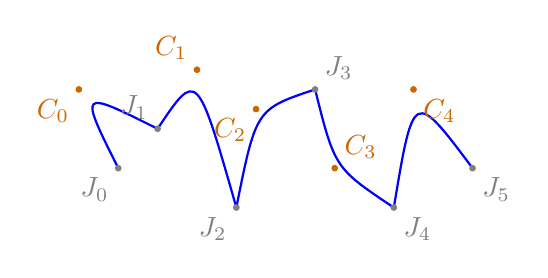
\begin{tikzpicture}[scale=0.5]
                    \coordinate (P0) at (0, 0);
                    \coordinate (P1) at (1, 1);
                    \coordinate (P2) at (3, -1);
                    \coordinate (P3) at (5, 2);
                    \coordinate (P4) at (7, -1);
                    \coordinate (P5) at (9, 0);

                    \coordinate (C0) at (-1, 2);
                    \coordinate (C1) at (2, 2.5);
                    \coordinate (C2) at (3.5, 1.5);
                    \coordinate (C3) at (5.5, 0);
                    \coordinate (C4) at (7.5, 2);

                    %\draw[gray, dashed] (P0) -- (P1) -- (P2) -- (P3) -- (P4) -- (P5);

                    \draw[thick, blue]   (P0) .. controls (C0) .. (P1);
                    \draw[thick, blue]   (P1) .. controls (C1) .. (P2);
                    \draw[thick, blue]   (P2) .. controls (C2) .. (P3);
                    \draw[thick, blue]   (P3) .. controls (C3) .. (P4);
                    \draw[thick, blue]   (P4) .. controls (C4) .. (P5);

                    \filldraw[white!50!black] (P0) circle (2pt) node[below left] {$J_0$};
                    \filldraw[white!50!black] (P1) circle (2pt) node[above left] {$J_1$};
                    \filldraw[white!50!black] (P2) circle (2pt) node[below left] {$J_2$};
                    \filldraw[white!50!black] (P3) circle (2pt) node[above right] {$J_3$};
                    \filldraw[white!50!black] (P4) circle (2pt) node[below right] {$J_4$};
                    \filldraw[white!50!black] (P5) circle (2pt) node[below right] {$J_5$};

                    \filldraw[orange!80!black] (C0) circle (2pt) node[below left] {$C_0$};
                    \filldraw[orange!80!black] (C1) circle (2pt) node[above left] {$C_1$};
                    \filldraw[orange!80!black] (C2) circle (2pt) node[below left] {$C_2$};
                    \filldraw[orange!80!black] (C3) circle (2pt) node[above right] {$C_3$};
                    \filldraw[orange!80!black] (C4) circle (2pt) node[below right] {$C_4$};

                \end{tikzpicture}
            \end{figure}
        \end{column}

        \begin{column}{5.5cm}
            \begin{figure}[h!]
                \centering
                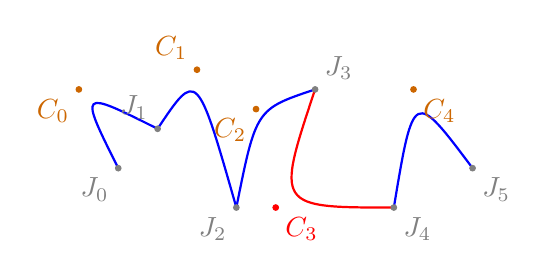
\begin{tikzpicture}[scale=0.5]
                    \coordinate (P0) at (0, 0);
                    \coordinate (P1) at (1, 1);
                    \coordinate (P2) at (3, -1);
                    \coordinate (P3) at (5, 2);
                    \coordinate (P4) at (7, -1);
                    \coordinate (P5) at (9, 0);

                    \coordinate (C0) at (-1, 2);
                    \coordinate (C1) at (2, 2.5);
                    \coordinate (C2) at (3.5, 1.5);
                    \coordinate (C3) at (4, -1);
                    \coordinate (C4) at (7.5, 2);

                    %\draw[gray, dashed] (P0) -- (P1) -- (P2) -- (P3) -- (P4) -- (P5);

                    \draw[thick, blue]   (P0) .. controls (C0) .. (P1);
                    \draw[thick, blue]   (P1) .. controls (C1) .. (P2);
                    \draw[thick, blue]   (P2) .. controls (C2) .. (P3);
                    \draw[thick, red]   (P3) .. controls (C3) .. (P4);
                    \draw[thick, blue]   (P4) .. controls (C4) .. (P5);

                    \filldraw[white!50!black] (P0) circle (2pt) node[below left] {$J_0$};
                    \filldraw[white!50!black] (P1) circle (2pt) node[above left] {$J_1$};
                    \filldraw[white!50!black] (P2) circle (2pt) node[below left] {$J_2$};
                    \filldraw[white!50!black] (P3) circle (2pt) node[above right] {$J_3$};
                    \filldraw[white!50!black] (P4) circle (2pt) node[below right] {$J_4$};
                    \filldraw[white!50!black] (P5) circle (2pt) node[below right] {$J_5$};

                    \filldraw[orange!80!black] (C0) circle (2pt) node[below left] {$C_0$};
                    \filldraw[orange!80!black] (C1) circle (2pt) node[above left] {$C_1$};
                    \filldraw[orange!80!black] (C2) circle (2pt) node[below left] {$C_2$};
                    \filldraw[red] (C3) circle (2pt) node[below right] {$C_3$};
                    \filldraw[orange!80!black] (C4) circle (2pt) node[below right] {$C_4$};

                \end{tikzpicture}
            \end{figure}
        \end{column}

    \end{columns}
        \vspace{1em}
        \item Additionally, this alleviates the issue of a high polynomial degree
    \end{itemize}
\end{frame}


\begin{frame}{B\'ezier splines: Continuity}
    \begin{itemize}
        \item In the previous example the curve is not very smooth\vspace{0.8em}
        \item To fix that, we introduce the notion of \textbf{continuity} \vspace{0.8em}
        \item B\'ezier splines can have different levels of continuity at the joint
        \vspace{0.8em}
        \begin{itemize}
            \item $C^0$-continuity refers to adjacent Bézier curves ending and starting at the same point
            \item $C^1$-continuity requires $C^0$-continuity and matching first derivative vectors at the joint
            \item $C^2$-continuity requires $C^1$-continuity and matching second derivative vectors at the joint
        \end{itemize}
        \vspace{0.8em}
        \item For \textbf{smooth curves}, $C^2$-continuity is required
    \end{itemize}
\end{frame}

\begin{frame}{B-splines}
    \begin{itemize}
        \item \strong{B-splines} (basis splines) are $C^2$-continuous B\'ezier splines \vspace{0.5em}
        \item B-splines of order $k$ are polynomial basis functions for splines of the same order, where, any spline can be represented as a linear combination of B-splines  \vspace{0.5em}
        \item Additionally, there exists a unique combination of B-splines for any given spline (de Boor, 1978) \vspace{0.5em}
        \item B-splines are fitting candidates for performing the so-called \textbf{spline interpolation} \vspace{0.2em}
        \end{itemize}
\end{frame}

\begin{frame}{B-splines: Spline interpolation}
    \begin{itemize}
        \item Spline interpolation is used to approximate functions by fitting splines, rather than using a single high-degree polynomial curve \vspace{0.2em}
        \item This process arises naturally from the formal definition of B-splines: it recursively defines each basis from a knot vector (Kaihuai, 1998),
        which indicates the positions where the splines should be connected \vspace{0.2em}
        \item Given \strong{grid G} we define a spline $S$ of $k^{\text{th}}$ order as:
            $$S_{k,G}(x) = \sum_i c_i B_{i,k}(x), \text{ where } $$
          $c_i$ are the \strong{coefficients} and $B_{i,k}(x)$ are the corresponding basis functions \vspace{0.2em}
          \begin{itemize}
            \item Liu et al. call grid what is usually called a uniform knot vector and coefficients what are usually called control points
          \end{itemize}
        \item This process maximizes pre-computed elements (\textit{minimizing possible learnable parameters})
    \end{itemize}
\end{frame}

\begin{frame}{B-splines and KANs}
    \begin{itemize}
        \item In KANs, each activation function is a $k^{\text{th}}$ order B-spline, with a $G$-valued and uniformly spaced grid  \vspace{0.3em}
        \item For each activation function what is left to learn is the coefficients of the spline \vspace{0.3em}
        \item Note that KAN also extends the grid on the edges of the spline, so that each grid point is influenced from the same number of polynomials \vspace{0.3em}
        \item Thus, for a KAN of width $W$ and depth $D$ the $\#$training parameters is $\mathbb{O}(W^2DG)$ \vspace{0.3em}
        \item The respective number of parameters for an MLP is $\mathbb{O}(W^2D)$, but KAN promises convergence with smaller widths \vspace{0.3em}
    \end{itemize}
\end{frame}

\begin{frame}{KANs: Implementation details}
    The authors used a few (questionable) tricks to train the network for optimal performance: \vspace{0.5em}
    \begin{enumerate}
        \item \textit{Residual activation functions}:
        $$\psi(x) = w_b\cdot silu(x) + w_s \cdot spline(x), \text{ where } spline(x) = \sum_i c_i B_i(x)$$
        \begin{center}
            \textit{\small \textcolor{blue!50!black}{(One can argue that this introduction of weights does not align with the initial claim)}} \vspace{1em}
        \end{center}
        \item \textit{Initialization scales}: The network's training is sensitive to initialization, so an optimal setup is introduced \vspace{1em}
    \end{enumerate}
\end{frame}



\section{Why Kolmogorov-Arnold Networks?}
{
  \setbeamertemplate{headline}{}
  \begin{frame}
    \sectionpage%
  \end{frame}
}

\begin{frame}{Grid extension}
    \begin{itemize}
        \item For learning a B-spline, more basis functions result in a finer-grained curve \vspace{0.5em}
        \item A very useful feature of KANs is their ability to at first learn a coarse curve for a specific number of
        grid points and then, at any point, resume the training with more grid points \vspace{0.5em}
        \item The network does not need to be re-trained, but instead they employ a smart idea:\vspace{1em}

        \begin{center}
            \textit{The coefficients of the fine-grained curve can be initialized from the coefficients of the coarse by minimizing
            the distance between the respective splines (over some distribution of input values)}
        \end{center}
    \end{itemize}
\end{frame}

\begin{frame}{Fixed activation functions}
    \begin{itemize}
        \item KANs also give the option instead of using learnable activation functions, to use \textbf{fixed symbolic functions} (polynomials, exponentials etc.) \vspace{1em}
        \item This is useful for problems where we have an intuition about their internal functions \vspace{1em}
        \item However, we cannot simply set the activation function to be the exact symbolic formula, since its inputs and outputs may have shifts and scalings \vspace{1em}
        \item So, in this case, the network learns the parameters of the affine transformation $$c \cdot \psi_{fixed}(a \cdot x_{in} + b) + d$$
    \end{itemize}
\end{frame}

\begin{frame}{Interpretability: Motivation}
    \begin{itemize}
        \item The main selling point of KANs is their interpretable structure, allowing \textbf{retrieval and examination of the learned activation functions} \vspace{0.5em}
        \item But, this is only useful when we a priori know the structure of the KAN and know what we expect to see \vspace{0.5em}
        \item For unknown problems, we stack KAN layers and experiment to find what works \vspace{0.5em}
        \item In this case, only some activation should be meaningful \vspace{0.5em}
        \item Then, how is the visualization considered interpretability? \vspace{0.5em}
        \item The idea is to start from a large enough KAN and train it with \strong{sparsity regularization followed by pruning}
    \end{itemize}
\end{frame}

\begin{frame}{Interpretability: Sparsification}
    \begin{itemize}
        \item In MLPs L1 regularization adds the absolute values of the model's weights to the loss function, promoting sparsity by encouraging smaller or zero weights \vspace{0.5em}
        \item Since KANs do not have linear weights, the L1-norm should be defined over the activation functions \vspace{0.5em}
        \item The L1 norm of an activation function ($\psi$) is its average magnitude over its inputs \vspace{0.5em}
        \item The L1 norm of a KAN layer ($\phi$) is the sum of L1 norms of all $\psi$'s \vspace{0.5em}
        \item Actually, L1-norm alone is insufficient, since the goal is to remove less informative or redundant features, not just to shrink weights, so an entropy penalty is introduced (layer-wise)\vspace{0.5em}
        \item So, the total training objective is the prediction loss plus L1 and entropy regularization of all KAN layers \vspace{0.5em}
    \end{itemize}
\end{frame}

\begin{frame}{Interpretability: Pruning}
    \begin{itemize}
        \item After training with sparsification penalty, we can prune the network to a smaller subnetwork \vspace{0.5em}
        \item The incentive is to throw away the unimportant activation functions \vspace{0.5em}
        \item For each node, its incoming score is defined as the maximum L1 norm of the outputs of the prior KAN layer \vspace{0.5em}
        \item Its outgoing score is defined as the maximum L1 norm of the outputs of the current KAN layer \vspace{0.5em}
        \item A node is considered to be important if \textbf{both incoming and outgoing scores are greater than a threshold hyperparameter} \vspace{0.5em}
    \end{itemize}
\end{frame}

\begin{frame}{Interpretability: Example}
    \begin{columns}
        \begin{column}{6cm}
            \begin{center}
                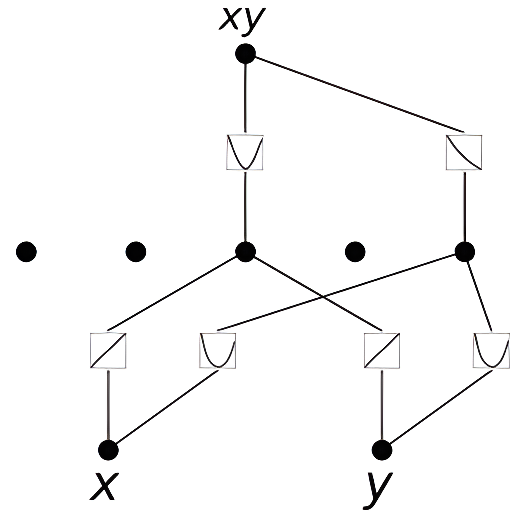
\includegraphics[width=5cm]{contents/images/pruning_example}
            \end{center}
        \end{column}

        \begin{column}{6cm}
            \begin{itemize}
                \item Function to be learned $f(x,y) = xy$ \vspace{1em}
                \item KAN computes: $$(x+y)^2 - (x^2+y^2)$$
                \item Note that: $$(x+y)^2 - (x^2+y^2) = 2xy$$
            \end{itemize}
        \end{column}
    \end{columns}
\end{frame}

\begin{frame}{Beating the COD (?)}
   \begin{itemize}
       \item The \textbf{curse of dimensionality (COD)} refers to the exponential growth in volume associated with adding more dimensions to a space \vspace{0.3em}
       \item UAT tells us that theoretically, a neural network with one hidden layer can approximate any function, but as the dimensionality of the input increases, the number of neurons required grows exponentially \vspace{0.3em}
       \item This leads to a MLP that is very large and potentially computationally intractable \vspace{0.3em}
       \item On the other hand, KAN's approximation ability is more dependent on the number of control points in each activation function and less on the data's dimension \vspace{0.3em}
       \item So, KAN's size will not increase exponentially as the data dimensions increase, but its grid should become more fine-grained \vspace{0.3em}
       \item However, we should note that the current implementation of KANs is not as optimized as the one for MLPs, so in practice the training times for high-dimensional data are comparable
   \end{itemize}
\end{frame}


\begin{frame}{Continual Learning}
   \begin{itemize}
       \item Catastrophic forgetting is a problem in MLPs \vspace{0.3em}
       \item When a MLPs is trained on one task and then  shifted to being trained on another, the network will soon forget about how to perform the first task \vspace{0.3em}
       \item Do you recall the motivation behind using splines to approximate curves instead of using polynomials? \strong{Locality!} \vspace{0.3em}
       \item Since spline bases are local, a sample will only affect a few nearby spline coefficients, leaving far-away coefficients intact \vspace{0.3em}
       \item This is desirable assuming faraway regions may have already stored information that we want to preserve \vspace{0.3em}
       \item By contrast, since MLPs usually use global activations any local change may propagate to regions far away \vspace{0.3em}
   \end{itemize}
\end{frame}

\section{Life after KAN}
{
  \setbeamertemplate{headline}{}
  \begin{frame}
    \sectionpage%
  \end{frame}
}

\begin{frame}{Extensions}
    \noindent
    \begin{center}
        \renewcommand{\arraystretch}{1.8}
        \setlength{\tabcolsep}{8pt}
        \begin{table}[ht]
            \centering
            \resizebox{0.98\textwidth}{!}{%
            \rowcolors{2}{brown!20}{white}
            \begin{tabular}{|p{6.5cm}|p{9cm}|p{3.3cm}|}
                \hline
                \rowcolor{brown!60}
                \textbf{Name} & \textbf{TLTR} & \textbf{Reference (2024)} \\ \hline
                KAN time series forecasting network & Vanilla KAN with shape [168,40,40,40,24] predicts 24 time-steps from 168 & Vaca-Rubio et al. \\ \hline
                Kolmogorov-Arnold Network Ordinary Differential Equations (KAN-ODEs) & Vanilla KAN used as an approximator for a dynamical system in the neural ODE framework & Koenig et al.\\ \hline
                Wavelet Kolmogorov-Arnold Networks (Wav-KAN) & KAN with shape [28x28,32,10] using wavelets instead of B-splines; Inputs are complete MNIST images & Bozorgasl and Chen \\ \hline
                Temporal Kolmogorov-Arnold Networks (TKAN) & Changes the output of the LSTM cell to $\sigma(\text{KAN}(x))$ & Genet and Inzirillo \\ \hline
            \end{tabular}%
            }
        \end{table}
    \end{center}
\end{frame}



\begin{frame}{Related Projects}

\strong{MANOLO: Explainability, computational efficiency}
%  
\begin{itemize}
\item Explore KANs as explainable models
\item Explore ways to reduce inefficiency
\end{itemize}

\vskip 1em

\strong{NavGreen: Maximizing efficiency of solar power usage}
%  
\begin{itemize}
\item Heat output, timeseries prediction
\item Modelling a physical phenomenon, KAN might outperform Transformer
\end{itemize}

\vskip 1em

\strong{Christoforos' MSc thesis:}
%  
\begin{itemize}
\item Using prior domain knowledge as KAN activation functions
\end{itemize}

\end{frame}



\begin{frame}{Plans}

\begin{itemize}
\item Deeper integration of KAN and recursive time-series
  processing
\item Mix prior and learned activation functions
  \begin{itemize}
  \item Exploit prior knowledge where available
  \item Give network flexibility to select \& parameterize, but also
    to model residuals from scratch
  \end{itemize}
\item CL4-2025-03-DIGITAL-EMERGING-07:
  \begin{itemize}
  \item Formal reasoning, mathematical problem-solving, confidence
    level estimation, long-term planning, and seamless adaptation to
    dynamic environments
  \item Continual learning, seamlessly adapt, learn from changing
    conditions, and retain knowledge essential for operation in
    dynamic, real-world environments
  \item Explainable AI and Trustworthy Decision-Making: causal
    inference, transparency, accountability
  \end{itemize}
\end{itemize}

\end{frame}



\section{The End}
% No section page needed, I think

\begin{frame}

\begin{center}
  \huge \colorbf{Thank you!} 
  Questions?
\end{center}

\vfill

\begin{columns}
\begin{column}{6cm}

\includegraphics[width=5cm]{fqsstyle/assets/deg} \\
\end{column}
\begin{column}{6cm}
Code, bibliography, slides:\\
\url{https://github.com/data-eng/kan}
\end{column}
\end{columns}

\end{frame}


\end{document}

